%
% $RCSfile: physical_architecture.tex,v $
%
% Copyright (C) 2002-2008. Christian Heller.
%
% Permission is granted to copy, distribute and/or modify this document
% under the terms of the GNU Free Documentation License, Version 1.1 or
% any later version published by the Free Software Foundation; with no
% Invariant Sections, with no Front-Cover Texts and with no Back-Cover
% Texts. A copy of the license is included in the section entitled
% "GNU Free Documentation License".
%
% http://www.cybop.net
% - Cybernetics Oriented Programming -
%
% http://www.resmedicinae.org
% - Information in Medicine -
%
% Version: $Revision: 1.1 $ $Date: 2008-08-19 20:41:08 $ $Author: christian $
% Authors: Christian Heller <christian.heller@tuxtax.de>
%

\chapter{Physical Architecture}
\label{physical_architecture_heading}
\index{Physical Architecture}
\index{Communication}
\index{Autonomous Systems}
\index{Interaction and Cooperation}
\index{Technical Systems}
\index{Computer}
\index{Client}
\index{Server}
\index{Communication Partners}
\index{System Constellations}
\index{Communication Languages}
\index{Information Technology Environment}
\index{IT}

\begin{flushright}
    \textsl{Simplicity is the Result of Maturity.}\\
    \textsc{Johann Christoph Friedrich von Schiller}
\end{flushright}

Software provides the functionality through which robots act and computers
represent and process information. Both are special kinds of machines which only
get useful for humans if they can be controlled and communicated with.
\emph{Communication} is an essential ability for almost any kind of system.
\emph{Autonomous} systems exist and may well be useful, but is it nearly always
the \emph{Interaction} and \emph{Cooperation} that makes technical systems (from
now on called \emph{Computer} in this work) so interesting and helpful to humans.

In many cases, systems are limited to one role: \emph{Client} or \emph{Server}.
Clients ask questions which servers answer. But both are able to send as well
as to receive information. One-way communication without any feedback is rarely
useful. Besides the mentioned client- and server-, there are other roles that a
computer system can take on when talking with so-called
\emph{Communication Partners}.

The following sections will stepwise build up- and briefly investigate some
examples of well-known system constellations and possible communication
languages that are commonly used in a general \emph{Information Technology}
(IT) environment. Because physical systems and their interactions are
considered without any knowledge about their inside, one also talks of this as
the \emph{Physical Architecture} of an IT environment. Its understanding is
important for later reflections on the inner architecture of software systems
(chapter \ref{logical_architecture_heading}). Also will chapter
\ref{state_and_logic_heading} come back to system communication principles and
introduce a translator architecture for universal communication.

%
% $RCSfile: process.tex,v $
%
% Copyright (C) 2002-2008. Christian Heller.
%
% Permission is granted to copy, distribute and/or modify this document
% under the terms of the GNU Free Documentation License, Version 1.1 or
% any later version published by the Free Software Foundation; with no
% Invariant Sections, with no Front-Cover Texts and with no Back-Cover
% Texts. A copy of the license is included in the section entitled
% "GNU Free Documentation License".
%
% http://www.cybop.net
% - Cybernetics Oriented Programming -
%
% http://www.resmedicinae.org
% - Information in Medicine -
%
% Version: $Revision: 1.1 $ $Date: 2008-08-19 20:41:08 $ $Author: christian $
% Authors: Christian Heller <christian.heller@tuxtax.de>
%

\section{Process}
\label{process_heading}
\index{Process}
\index{Resource Grouping}
\index{Execution}
\index{Address Space}
\index{Thread of Execution}
\index{Central Processing Unit}
\index{CPU}
\index{Program Counter}
\index{Registers}
\index{Stack}
\index{Abstract System Concepts}
\index{Operating System}
\index{OS}
\index{Session}
\index{Process Group}
\index{Job}
\index{System}
\index{Application}
\index{Task}
\index{Lightweight Process}
\index{Work Queue}
\index{Task Farm}
\index{Task Bag}

The most common word used to describe a running computer program is
\emph{Process}. Tanenbaum \cite{tanenbaum2001} defines it as an abstract model
based on two independent concepts: \emph{Resource Grouping} (space) and
\emph{Execution} (time).

He writes that \emph{Resource Grouping} meant that a process had an address
space containing program text and data, as well as other resources. A
\emph{Thread of Execution}, on the other hand, were the entity scheduled for
execution on the \emph{Central Processing Unit} (CPU). It had a program counter
(keeping track of which instruction to execute next), registers (holding its
current working variables) and a stack (containing the execution history, with
one frame for each procedure called but not yet returned from). Although a
thread would have to execute in some process, the thread and its process were
different concepts and could be treated separately.

A slightly different explanation is given in \cite{iseries}:

\begin{quote}
    A thread is the path a program takes while it runs, the steps it performs,
    and the order in which it performs the steps. A thread runs code from its
    starting location in an ordered, predefined sequence for a given set of
    inputs. The term \emph{Thread} is shorthand for \emph{Thread of Control}.
    (One) can use multiple threads to improve application performance by
    running different application tasks simultaneously.
\end{quote}

\begin{table}[ht]
    \begin{center}
        \begin{footnotesize}
        \begin{tabular}{| p{25mm} | p{45mm} | p{35mm} |}
            \hline
            \textbf{Abstract Concept} & \textbf{Explanation} & \textbf{Synonyms}\\
            \hline
            Session & Bundle of processes of one user &\\
            \hline
            Process Group & Collection of one or more processes & Job\\
            \hline
            Process & Container for related Resources & System, Application, Task\\
            \hline
            Thread & Schedulable Entity & Lightweight Process\\
            \hline
        \end{tabular}
        \end{footnotesize}
        \caption{Systematics of Abstract System Concepts}
        \label{concepts_table}
    \end{center}
\end{table}

There are other abstract concepts which are of importance, especially in an
\emph{Operating System} (OS) context. A terminal in the \emph{Linux} OS
\cite{johnson}, for example, may control a \emph{Session} consisting of
\emph{Process Groups} which in turn contain many \emph{Processes} providing
resources for the threads running in them. Table \ref{concepts_table} shows one
possible systematics of these concepts.

Some ambiguities exist, however. The term \emph{Job} which, some decades ago,
still stood for a program or set of programs, is nowadays used to label a
process group in \emph{Windows 2000} \cite[p. 7, 796]{tanenbaum2001} and
similarly in \emph{Linux} \cite[p. 125, 237]{johnson}. The notion of a
\emph{Task} is sometimes used equivalent to thread \cite{daene}, but other
times refers to a process or even process group \cite[p. 113]{johnson}.
Additionally, some sources use the term in the meaning of a signal or event
belonging to a work queue called \emph{Task Farm} or \emph{Task Bag}
\cite[p. 548, 606]{tanenbaum1999}.

This document uses the more general word \emph{System} to write about a process
that manages the input, storage, processing and output of data in a computer.
This is contrary to some other works which mean a whole computer, including its
hardware and software programs running on it, when talking about systems. In
the understanding of this work, once again, a \emph{System} is a \emph{Process}
(software system) running on a \emph{Computer} (hardware system).

%
% $RCSfile: application_server.tex,v $
%
% Copyright (C) 2002-2008. Christian Heller.
%
% Permission is granted to copy, distribute and/or modify this document
% under the terms of the GNU Free Documentation License, Version 1.1 or
% any later version published by the Free Software Foundation; with no
% Invariant Sections, with no Front-Cover Texts and with no Back-Cover
% Texts. A copy of the license is included in the section entitled
% "GNU Free Documentation License".
%
% http://www.cybop.net
% - Cybernetics Oriented Programming -
%
% http://www.resmedicinae.org
% - Information in Medicine -
%
% Version: $Revision: 1.1 $ $Date: 2008-08-19 20:41:05 $ $Author: christian $
% Authors: Christian Heller <christian.heller@tuxtax.de>
%

\section{Application Server}
\label{application_server_heading}
\index{Application Server}
\index{Presentation Clients}
\index{Standalone Systems}
\index{Operating System}
\index{OS}
\index{Layers}
\index{Tier}
\index{1 Tier}
\index{n Tier}
\index{Server Process}
\index{Server}
\index{Client}

One well-known system, nowadays, is the \emph{Application Server}. The name
implies that this system is to \emph{serve} other systems, so-called
\emph{Presentation Clients} (section \ref{presentation_client_heading}). It may
be programmed in languages like \emph{Java}, \emph{Python}, \emph{Smalltalk},
\emph{C++}, \emph{C} or others more.

On the other hand, there are systems running all by themselves, without any
access to/ from another system -- so-called \emph{Standalone Systems}. In
reality, they hardly exist since most applications run in a surrounding
\emph{Operating System} (OS) and are thus not really \emph{alone}. An OS may be
called \emph{standalone} but mostly, even that consists of a number of sub
processes solving background tasks. That is why the name \emph{standalone} is
used when one wants to place emphasis on the system itself, neglecting its
communication with others.

Many kinds of application servers exist. Multiple services are offered by them,
for example storage or persistence handling but also application- and domain
specific functionality. A healthcare environment, as example, may contain several
servers, each fulfilling one task such as person identification, resource access
decision, image access and so on -- just like people in real life have abilities
and professions.

Systems of an IT environment are structured into so-called \emph{Layers},
another name for which is \emph{Tier}. The application server alone represents
a \emph{1 Tier} environment. The more systems of different type (presentation
client, application server, database server) are added to an environment, the
more tiers are added. For that reason, distributed client-server environments
are called \emph{n Tier}.

When people talk about a \emph{Server}, they very often mean a \emph{Computer}
on which a \emph{Server Process} is running. This is neither completely wrong nor
absolutely correct. A computer can run many different processes, only some of
which may be servers. Hence, the computer can act as \emph{Server} but also as
\emph{Client}, at the same time.

%
% $RCSfile: database_server.tex,v $
%
% Copyright (C) 2002-2008. Christian Heller.
%
% Permission is granted to copy, distribute and/or modify this document
% under the terms of the GNU Free Documentation License, Version 1.1 or
% any later version published by the Free Software Foundation; with no
% Invariant Sections, with no Front-Cover Texts and with no Back-Cover
% Texts. A copy of the license is included in the section entitled
% "GNU Free Documentation License".
%
% http://www.cybop.net
% - Cybernetics Oriented Programming -
%
% http://www.resmedicinae.org
% - Information in Medicine -
%
% Version: $Revision: 1.1 $ $Date: 2008-08-19 20:41:06 $ $Author: christian $
% Authors: Christian Heller <christian.heller@tuxtax.de>
%

\section{Database Server}
\label{database_server_heading}
\index{Database Server}
\index{Database Management System}
\index{DBMS}
\index{Database}
\index{DB}
\index{2 Tiers}
\index{Persistent Data}
\index{Transient Data}
\index{Querying}
\index{Transaction Handling}
\index{Locking}
\index{Hierarchical DBMS}
\index{Network DBMS}
\index{Relational DBMS}
\index{RDBMS}
\index{Object-Relational DBMS}
\index{ORDBMS}
\index{Object-Oriented DBMS}
\index{OODBMS}
\index{Data Definition Language}
\index{DDL}
\index{Structured Query Language}
\index{SQL}
\index{Object-Relational DBMS}
\index{Object-Oriented Model}
\index{OOM}
\index{Entity-Relationship Model}
\index{ERM}
\index{Object Query Language}
\index{OQL}
\index{Middleware}
\index{Java Database Connectivity}
\index{JDBC}
\index{Open Database Connectivity}
\index{ODBC}
\index{Enterprise Java Beans}
\index{EJB}
\index{Business Objects}
\index{BO}

Another popular kind of server system, besides the application server, is the
\emph{Database Server}, also called \emph{Database Management System} (DBMS).
It manages structured data called a \emph{Database} (DB) and serves clients
with \emph{persistent} data. The arrow in figure \ref{database_figure} points
in the direction into which the application server sends its queries to the
database server, in order to retrieve data. Example DBMS representatives are
\emph{PostgreSQL}, \emph{MySQL}, \emph{DB2}, \emph{ORACLE}, \emph{ObjectStore},
\emph{POET} or \emph{Versant}.

\begin{figure}[ht]
    \begin{center}
        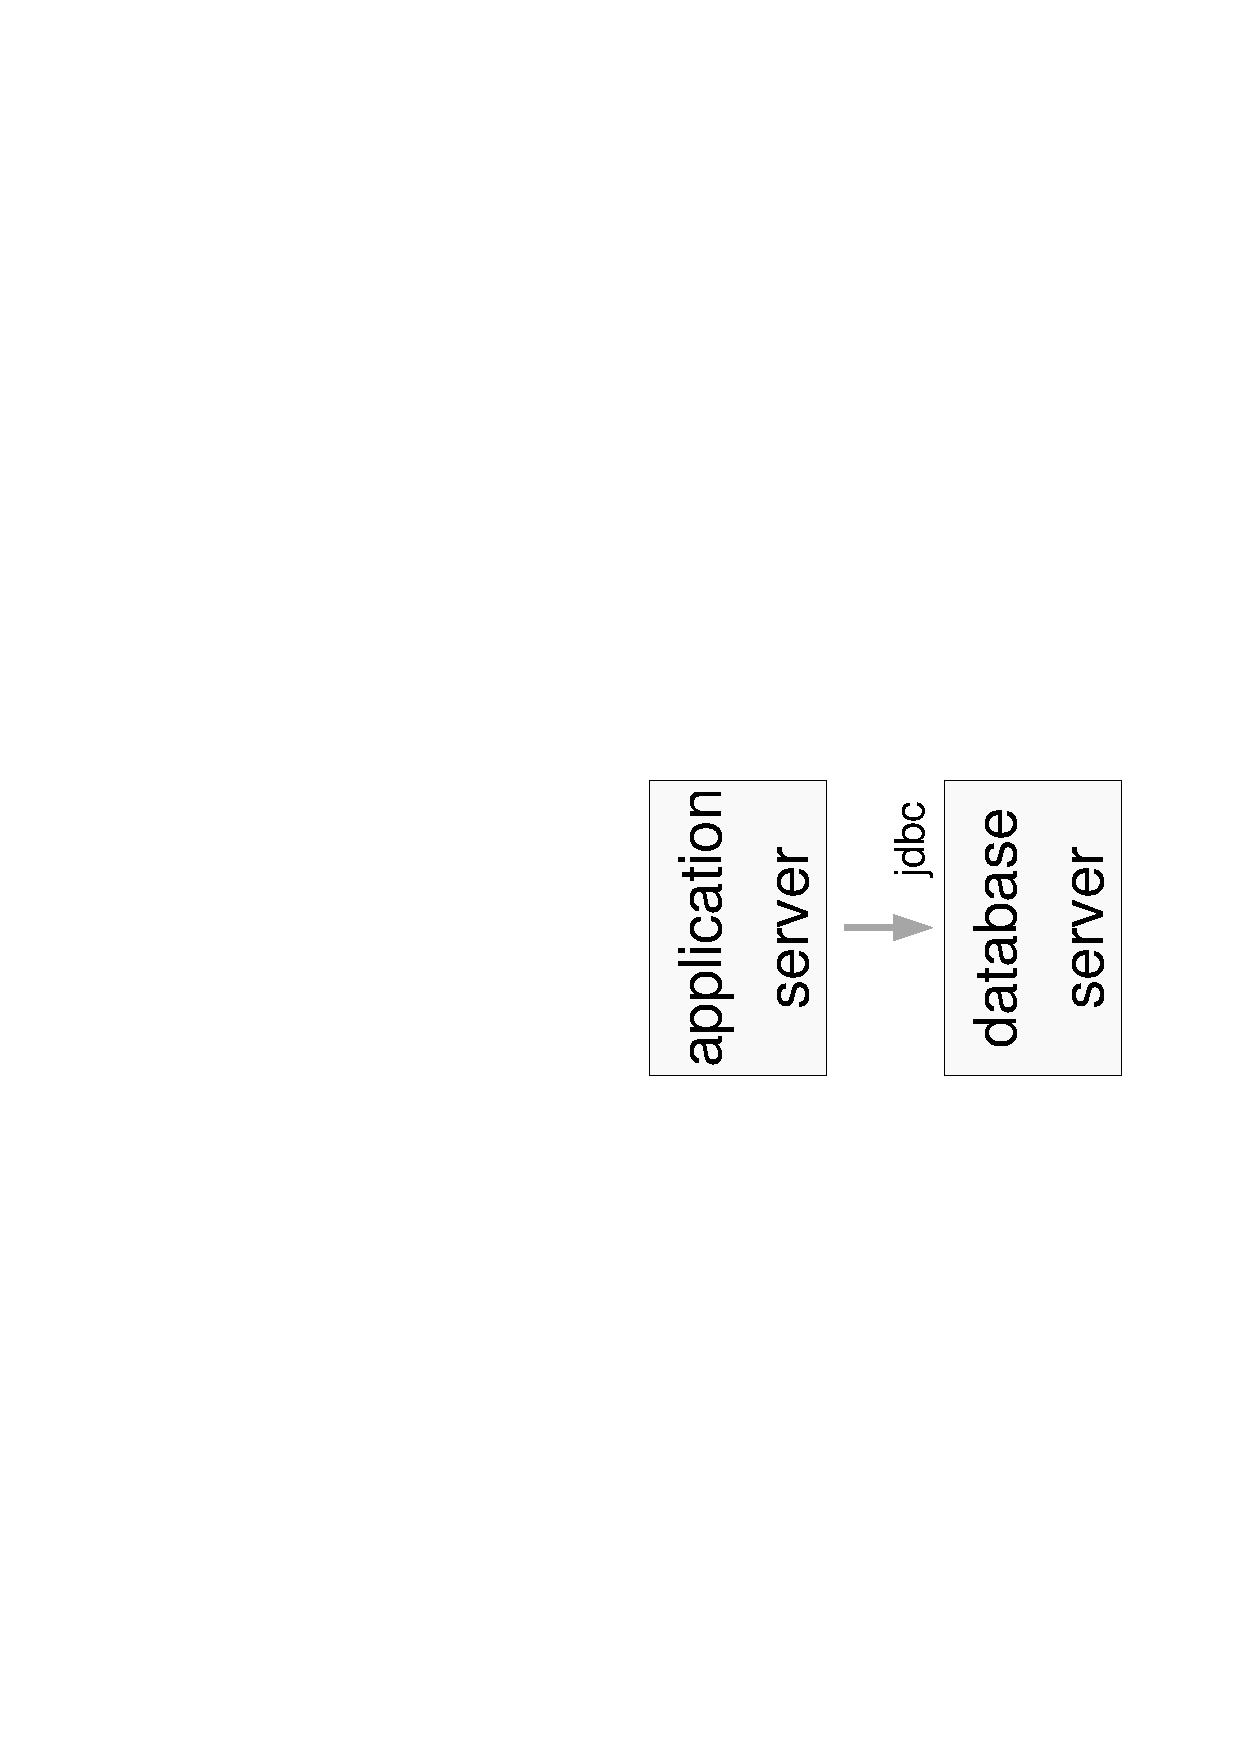
\includegraphics[scale=0.3,angle=-90]{graphic/database.pdf}
        \caption{Database Server (2 Tiers)}
        \label{database_figure}
    \end{center}
\end{figure}

\emph{Persistent Data} are those that live longer than the system working on them.
Very often, this is domain-specific- but also configuration information. These
are stored in a filesystem or database \cite{zimmermann}. \emph{Transient Data},
on the other hand, is temporary information that a system holds during its
lifetime, to function correctly. They get destroyed together with the system
which created them.

Managing persistent data implies a number of quite complex tasks, the details of
which will not be part of this document. To these aspects of database servers
belong:

\begin{itemize}
    \item[-] Querying
    \item[-] Transaction Handling
    \item[-] Locking
\end{itemize}

Different types of database systems exist. The major ones are:

\begin{itemize}
    \item[-] \emph{Hierarchical and Network DBMS}
    \item[-] \emph{Relational DBMS} (RDBMS)
    \item[-] \emph{Object-Relational DBMS} (ORDBMS)
    \item[-] \emph{Object-Oriented DBMS} (OODBMS)
\end{itemize}

Hierarchical DBMS were the first (electronic) databases ever used. They managed
their data in tree structures, starting each access from the root node. Network
DBMS went one step further: data could be associated at will \cite[p. 128]{zimmermann}.
Relational DBMS are based on tabular data structures which can have relations.
They were the first to accomplish a true separation between application and data.
Special languages were created to define and query such data sources: The
\emph{Data Definition Language} (DDL) and the \emph{Structured Query Language}
(SQL). Object-Relational DBMS were to fill the semantic gap between
\emph{Object-Oriented Model} (OOM) and \emph{Entity-Relationship Model} (ERM)
structures. Their extensions introduced a number of user-defined data types.
Object-Oriented DBMS conclusively close the semantic gap between object-oriented
applications and data. Their programming interface is often integrated into a
framework. The new SQL-based \emph{Object Query Language} (OQL)
\cite[p. 138]{zimmermann} was created for them.

The communication between systems can be eased with special techniques. After
Tanenbaum \cite{tanenbaum2002}, these were often called \emph{Middleware} since
they are placed between a higher-level layer consisting of users and applications,
and a layer underneath consisting of operating systems. In the case of database
systems, one such mechanism is the \emph{Java Database Connectivity} (JDBC)
\cite{hamilton, klute}; another one the \emph{Open Database Connectivity}
(ODBC) \cite[p. 170, 177]{zimmermann}. They provide a common interface for many
different relational databases.

Another technique are \emph{Enterprise Java Beans} (EJB) and comparable mechanisms.
They represent so-called \emph{Business Objects} (BO) and hence actually belong
to the previous section describing application servers. However, the containers
in which EJBs live also contain functionality for persistence- and transaction
handling which is why they are mentioned here. Further documentation can be found
in the corresponding literature \cite{gruhn} and sources \cite{blueprints, java}.

%
% $RCSfile: presentation_client.tex,v $
%
% Copyright (C) 2002-2008. Christian Heller.
%
% Permission is granted to copy, distribute and/or modify this document
% under the terms of the GNU Free Documentation License, Version 1.1 or
% any later version published by the Free Software Foundation; with no
% Invariant Sections, with no Front-Cover Texts and with no Back-Cover
% Texts. A copy of the license is included in the section entitled
% "GNU Free Documentation License".
%
% http://www.cybop.net
% - Cybernetics Oriented Programming -
%
% http://www.resmedicinae.org
% - Information in Medicine -
%
% Version: $Revision: 1.1 $ $Date: 2008-08-19 20:41:08 $ $Author: christian $
% Authors: Christian Heller <christian.heller@tuxtax.de>
%

\section{Presentation Client}
\label{presentation_client_heading}
\index{Presentation Client}
\index{Client}
\index{3 Tiers}
\index{Remote Method Invocation}
\index{RMI}
\index{Remote Procedure Call}
\index{RPC}
\index{Thin Client}
\index{Fat Client}
\index{Rich Client}

A system is called \emph{Client} when it uses services of a server. Most modern
applications incorporate abilities to communicate with server systems which may
run on the same computer as the client or on a remote machine that has to be
accessed over network.

\begin{figure}[ht]
    \begin{center}
        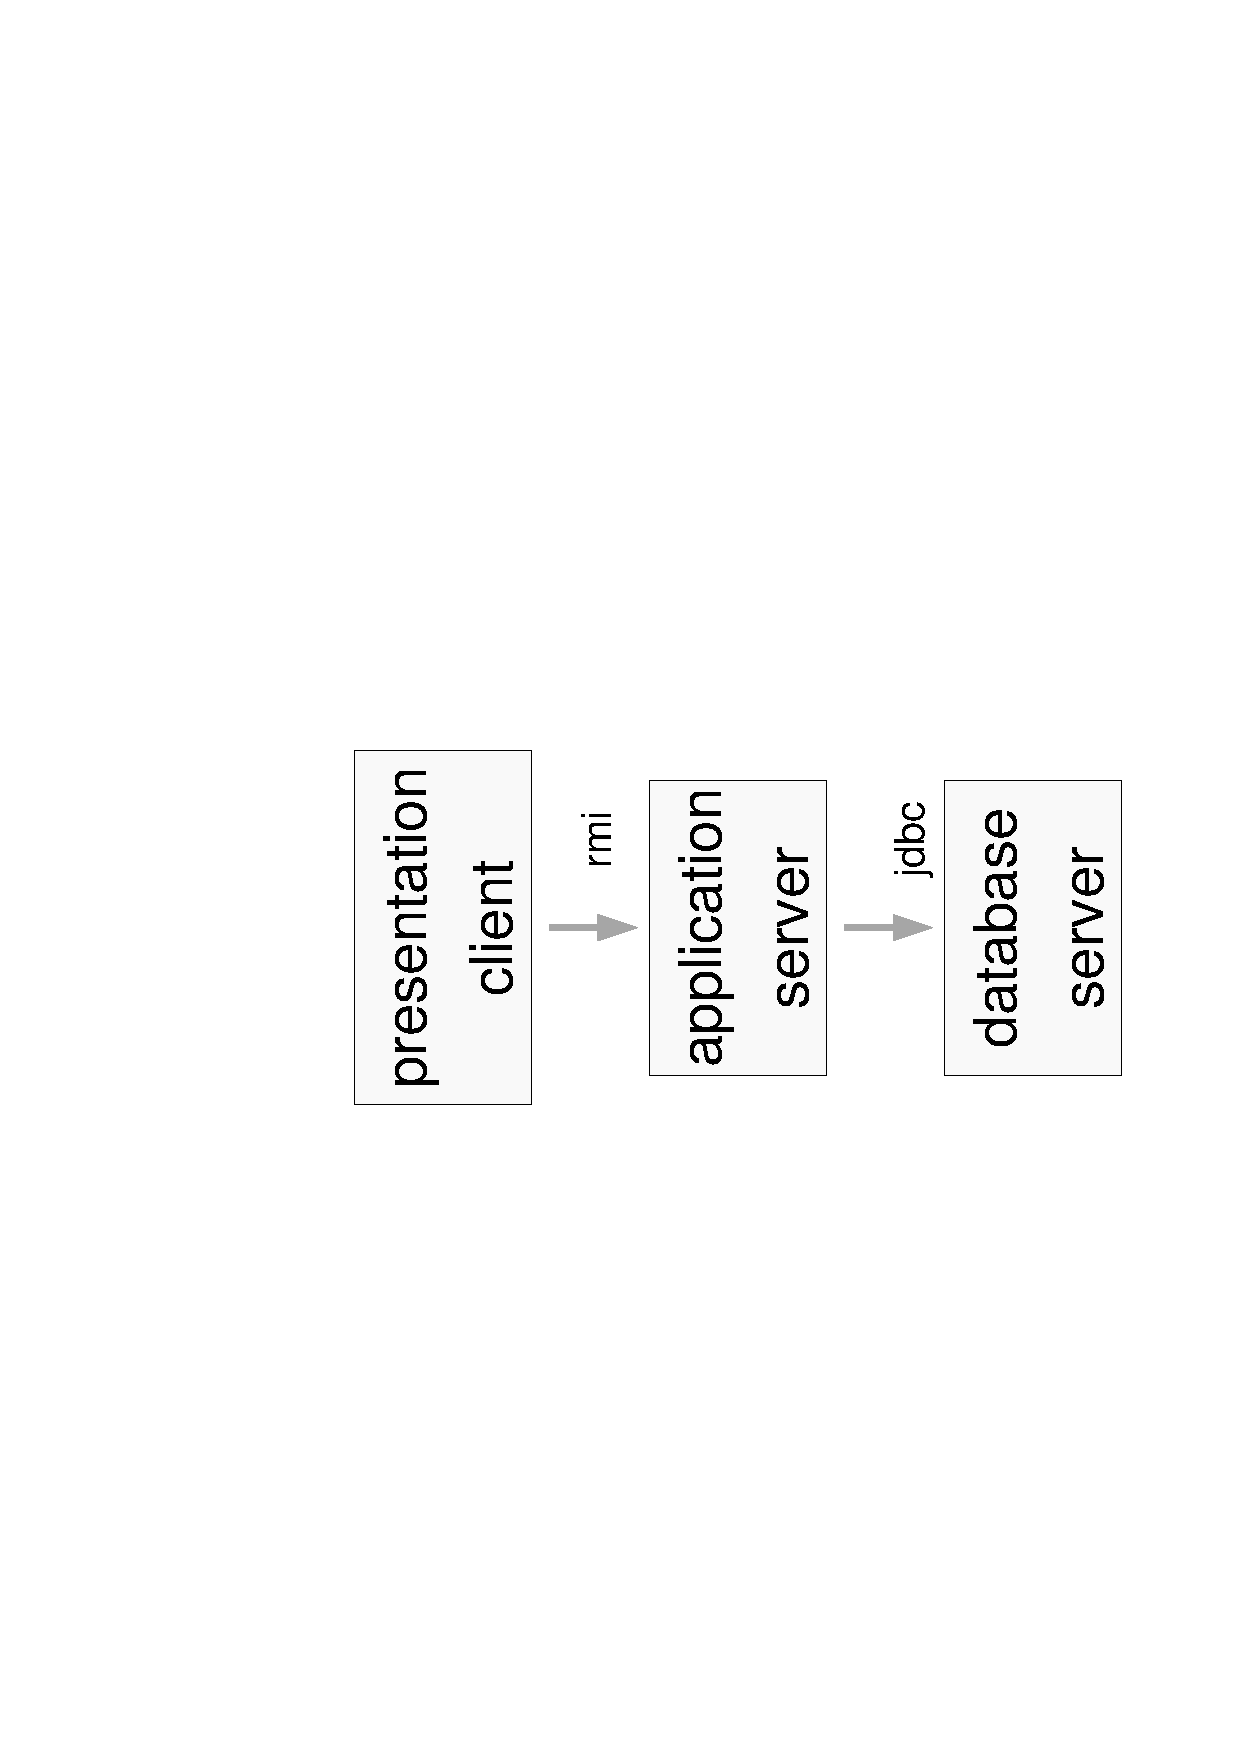
\includegraphics[scale=0.3,angle=-90]{graphic/client.pdf}
        \caption{Presentation Client (3 Tiers)}
        \label{client_figure}
    \end{center}
\end{figure}

But also clients can offer services as well as servers can use external services
and such become clients themselves. The application server in figure
\ref{database_figure} becomes a client when accessing the database system.
As can be seen -- \emph{Client} and \emph{Server} are quite arbitrary terms to
characterise systems.

Figure \ref{client_figure} illustrates the communication between a presentation
client and application server over network. Again, various mechanisms such as
\emph{Remote Method Invocation} (RMI), outside the Java world rather called
\emph{Remote Procedure Call} (RPC), exist to ease the way two remote systems
talk with one another.

Frequently, people distinguish between \emph{Thin Client} and \emph{Fat Client}
(the latter also called \emph{Rich Client}) \cite[p. 176]{zimmermann}. While a
thin client's task is nothing else than to display information coming from some
server, a fat client also takes over part of the business data processing which
is otherwise done by the server only.

%
% $RCSfile: web_client_and_server.tex,v $
%
% Copyright (C) 2002-2008. Christian Heller.
%
% Permission is granted to copy, distribute and/or modify this document
% under the terms of the GNU Free Documentation License, Version 1.1 or
% any later version published by the Free Software Foundation; with no
% Invariant Sections, with no Front-Cover Texts and with no Back-Cover
% Texts. A copy of the license is included in the section entitled
% "GNU Free Documentation License".
%
% http://www.cybop.net
% - Cybernetics Oriented Programming -
%
% http://www.resmedicinae.org
% - Information in Medicine -
%
% Version: $Revision: 1.1 $ $Date: 2008-08-19 20:41:09 $ $Author: christian $
% Authors: Christian Heller <christian.heller@tuxtax.de>
%

\section{Web Client and Server}
\label{web_client_and_server_heading}
\index{Web Client and Server}
\index{Internet}
\index{Web Server}
\index{Web Client}
\index{Web Browser}
\index{Applets}
\index{Servlets}
\index{Transfer Control Protocol}
\index{TCP}
\index{Internet Protocol}
\index{IP}
\index{Hypertext Transfer Protocol}
\index{HTTP}

With the emerge of the \emph{Internet}, several new kinds of services like
\emph{Email}, \emph{File Transfer}, \emph{Web} etc. became popular. The web
service allows information to be published in form of a \emph{Web Page}. Web
pages can be written in markup formats like \emph{Hypertext Markup Language}
(HTML) and \emph{Extensible Markup Language} (XML) or, using special tags, as
\emph{Java Server Pages-} (JSP) and \emph{PHP Hypertext Preprocessor-} (PHP)
instructions. Before being displayed, the latter two need to be translated by a
preprocessor inside the web server, into HTML.

\begin{figure}[ht]
    \begin{center}
        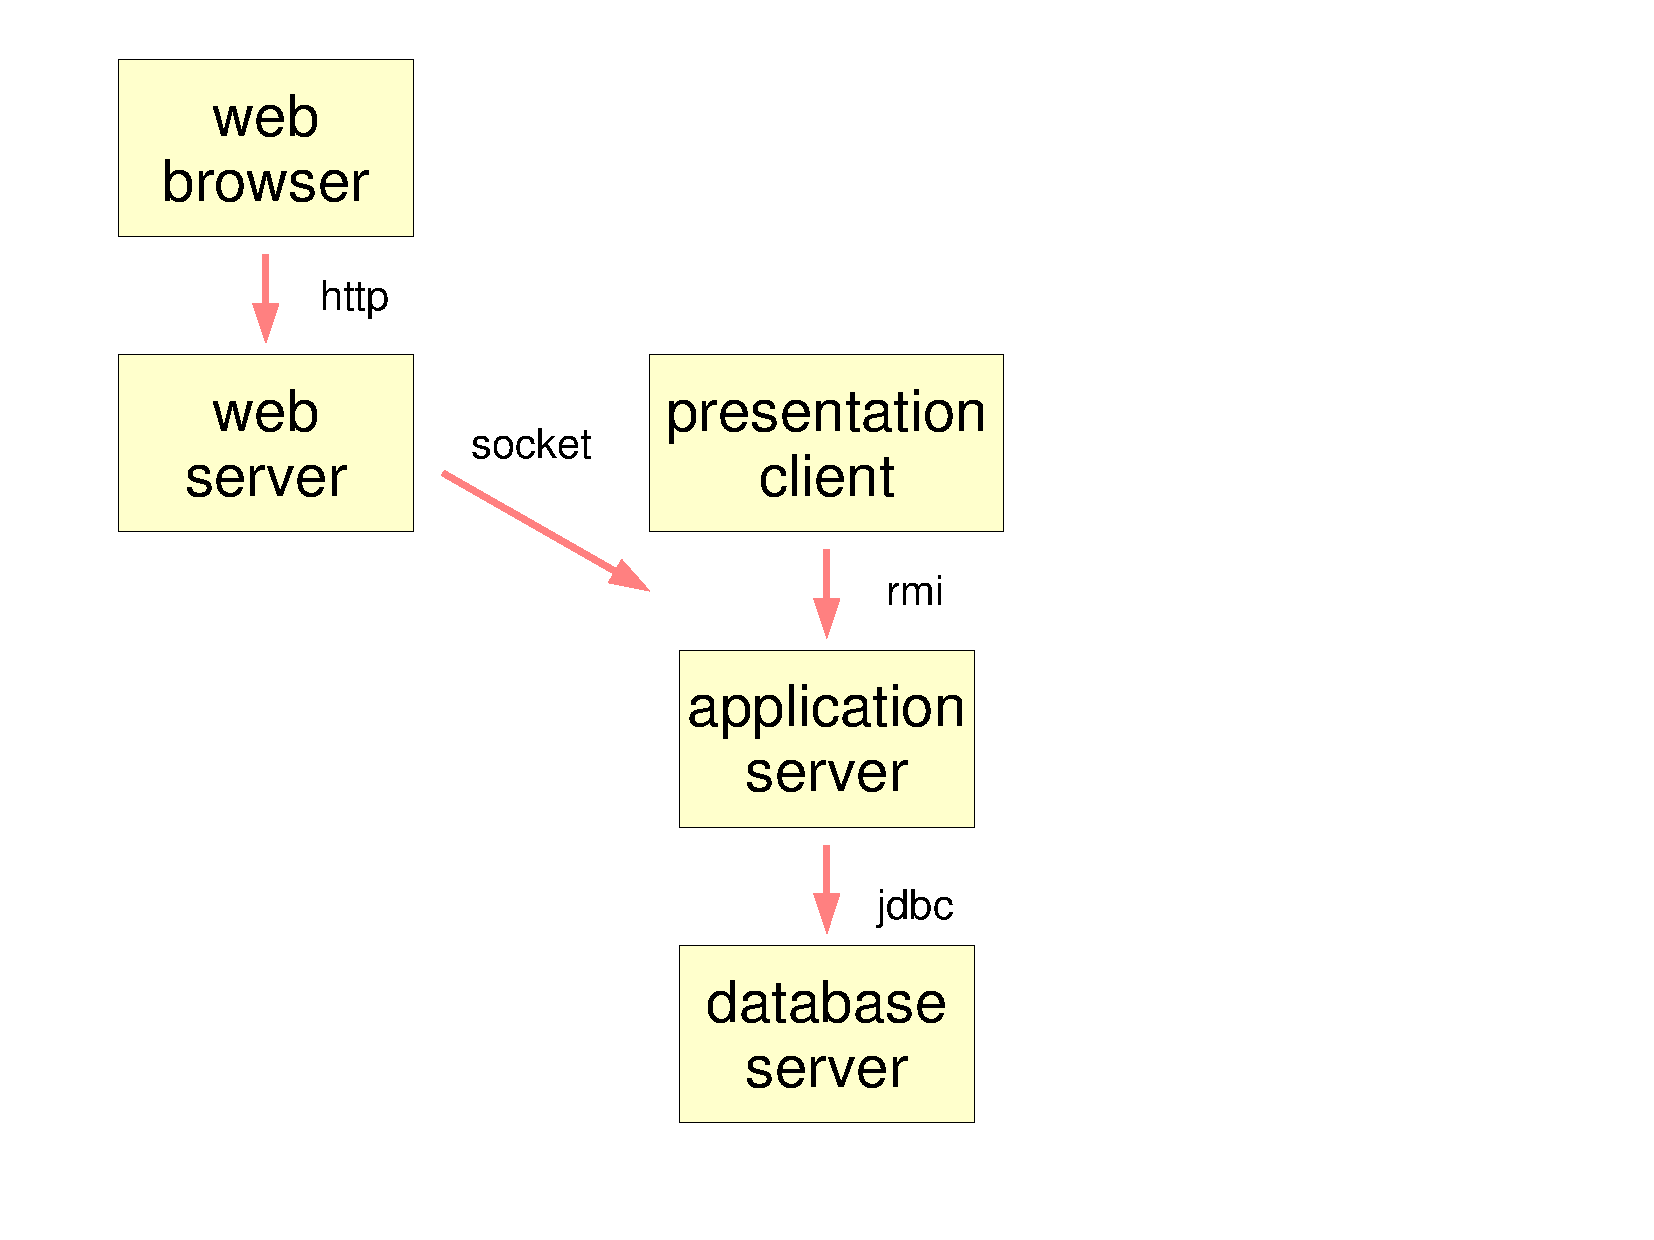
\includegraphics[scale=0.3,angle=-90]{graphic/web.pdf}
        \caption{Web Client and Server}
        \label{web_figure}
    \end{center}
\end{figure}

The principle as shown in figure \ref{web_figure} is easy: A \emph{Web Server}
stores web pages which can be accessed by clients called \emph{Web Browser}.
Browsers extract and translate (render) the (graphical) information given in
form of a web page and display them. But they are also able to handle actions
such as keyboard input or mouse click, and send these information back to the
web server.

Moreover, browsers can locally execute small programs called \emph{Applets}
which were downloaded from the web server. Their counterpart are \emph{Servlets}
which are executed in multiple threads on the web server, offering the actual
services.

Web communication is based on standards like the \emph{Transfer Control Protocol}/
\emph{Internet Protocol} (TCP/IP) and the \emph{Hypertext Transfer Protocol}
(HTTP) \cite{tanenbaum2000}. Section \ref{systems_interconnection_heading} will
systematise them together with other standards for system interconnection. The
socket mechanism may be used to connect a web server to an application server.

Many other aspects are important when talking about internet services. There is
the issue of security, there is performance, user-friendliness and many more
which will not be discussed further here, since it would exceed the frame of
this work.

%
% $RCSfile: local_process.tex,v $
%
% Copyright (C) 2002-2008. Christian Heller.
%
% Permission is granted to copy, distribute and/or modify this document
% under the terms of the GNU Free Documentation License, Version 1.1 or
% any later version published by the Free Software Foundation; with no
% Invariant Sections, with no Front-Cover Texts and with no Back-Cover
% Texts. A copy of the license is included in the section entitled
% "GNU Free Documentation License".
%
% http://www.cybop.net
% - Cybernetics Oriented Programming -
%
% http://www.resmedicinae.org
% - Information in Medicine -
%
% Version: $Revision: 1.1 $ $Date: 2008-08-19 20:41:07 $ $Author: christian $
% Authors: Christian Heller <christian.heller@tuxtax.de>
%

\section{Local Process}
\label{local_process_heading}
\index{Local Process}
\index{Nodes}
\index{Daemon}
\index{Small Servers}
\index{Inter-Process Communication}
\index{IPC}
\index{Dynamic Data Exchange}
\index{DDE}
\index{Object Linking and Embedding}
\index{OLE}
\index{ActiveX}
\index{Component Object Model}
\index{COM}
\index{Java Message Service}
\index{JMS}
\index{Desktop Communication Protocol}
\index{DCOP}
\index{Bonobo}
\index{Pipes}

Not all software systems run on physically separated computers, also called
\emph{Nodes}. And not all communication happens over network. As well, one
\emph{Local Process} can talk to a second on the same machine (figure
\ref{local_figure}). In fact, all applications have this ability, at least for
talking with the surrounding operating system.

\begin{figure}[ht]
    \begin{center}
        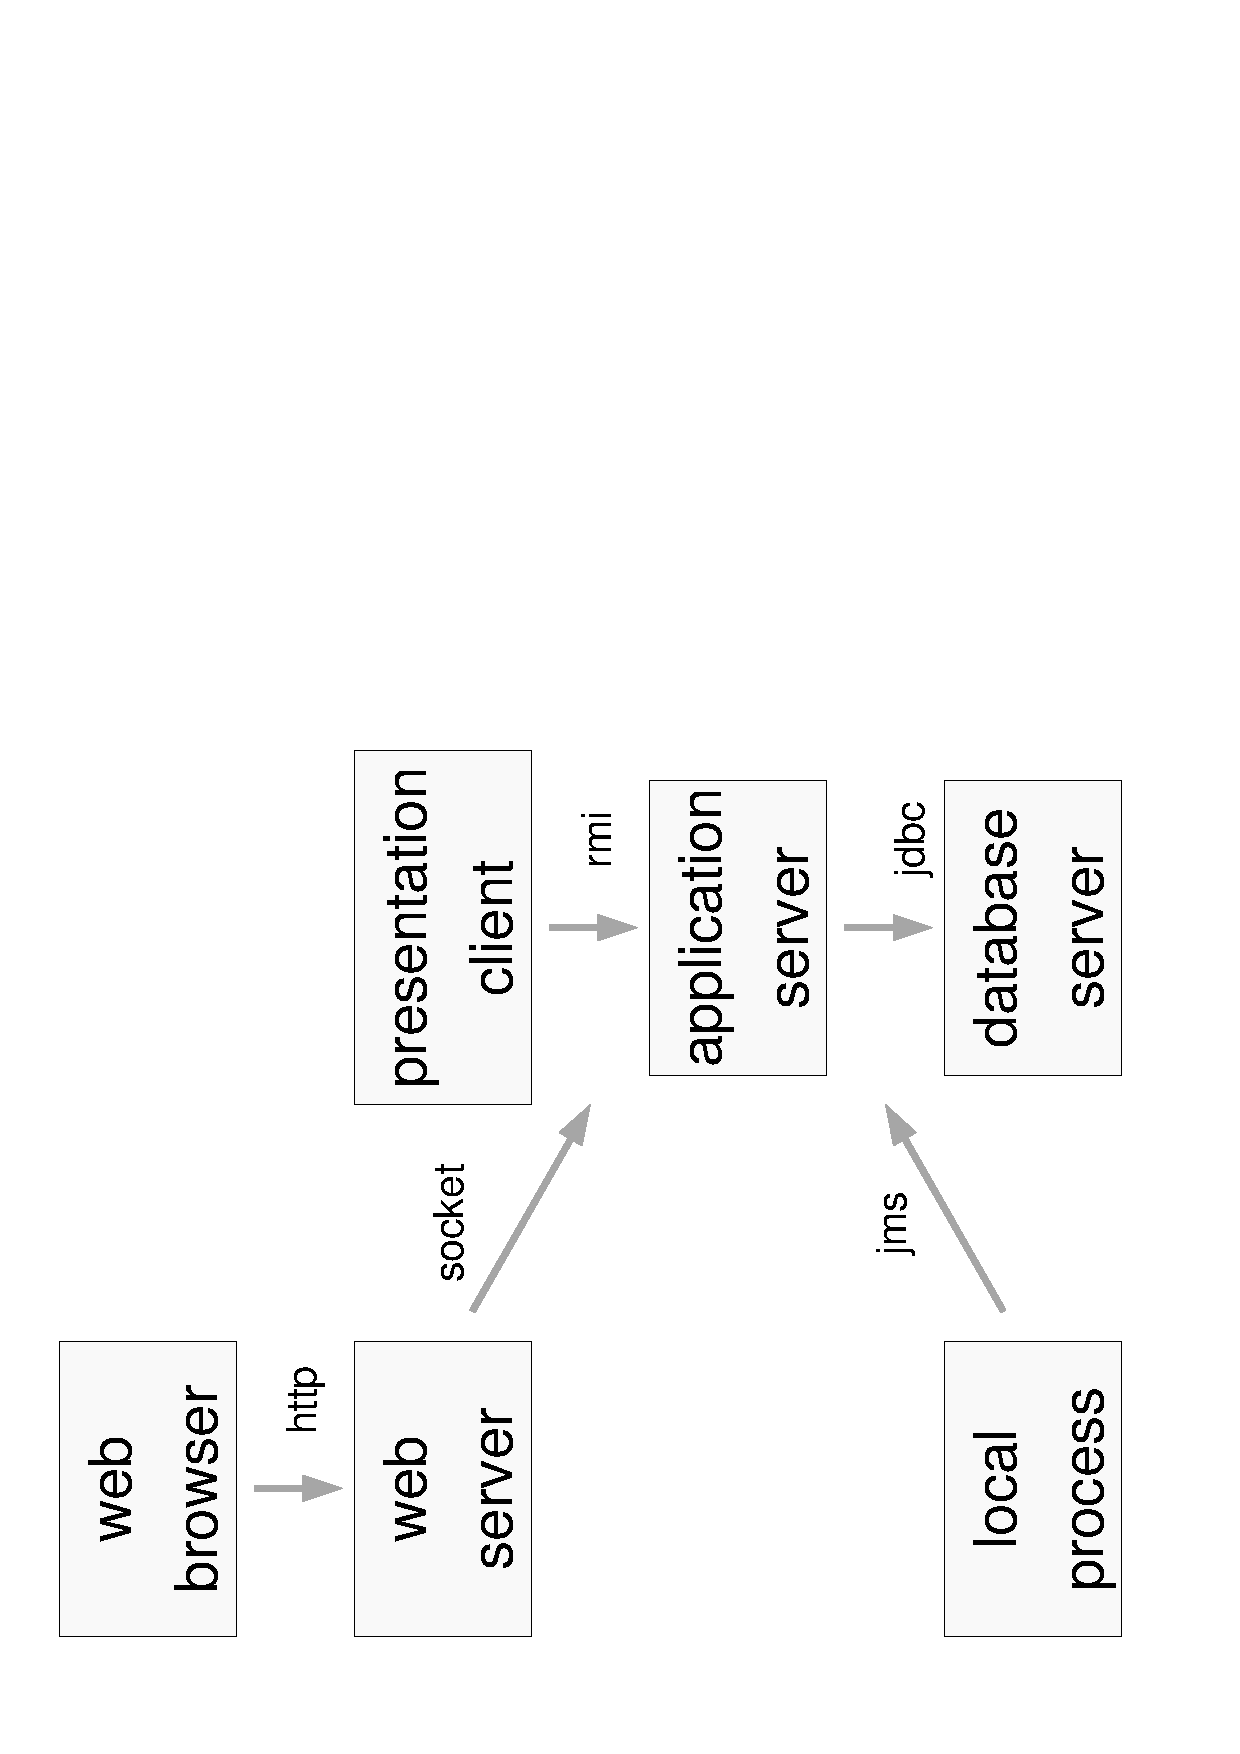
\includegraphics[scale=0.3,angle=-90]{graphic/local.pdf}
        \caption{Local Process}
        \label{local_figure}
    \end{center}
\end{figure}

Sometimes, local processes are needed by the operating system itself. Those are
running in the background then which is why they are often called \emph{Daemon}.
Because they offer special services, daemons are nothing else than small
servers. They fulfil tasks like managing all printing or email delivery of a
system, or similar things \cite[p. 74]{tanenbaum2001}.

Very often, it is useful to let local client applications talk with each other.
One part of a document (for instance a diagram) that was created by help of a
special application may want to get integrated into another document (for instance
a letter) which is edited by another application. A number of mechanisms were
created to solve this \emph{Inter-Process Communication} (IPC) task, for example:

\begin{itemize}
    \item[-] \emph{Dynamic Data Exchange} (DDE) \cite{ddefaq}
    \item[-] \emph{Object Linking and Embedding} (OLE/ OLE2) and \emph{ActiveX},
        both now based on the \emph{Component Object Model} (COM)
        \cite{zimmermann, gruhn}
    \item[-] \emph{Java Message Service} (JMS) \cite{java}
    \item[-] \emph{Desktop Communication Protocol} (DCOP) \cite{kde}
    \item[-] \emph{Bonobo} \cite{gnome}
    \item[-] \emph{Pipes} \cite{johnson, tanenbaum2001}
\end{itemize}

Although usually used for local communication (on the same node), some of these
also function over network. Again, this document will not discuss their inside
functionality. Plenty of books were written about that.

%
% $RCSfile: human_user.tex,v $
%
% Copyright (C) 2002-2008. Christian Heller.
%
% Permission is granted to copy, distribute and/or modify this document
% under the terms of the GNU Free Documentation License, Version 1.1 or
% any later version published by the Free Software Foundation; with no
% Invariant Sections, with no Front-Cover Texts and with no Back-Cover
% Texts. A copy of the license is included in the section entitled
% "GNU Free Documentation License".
%
% http://www.cybop.net
% - Cybernetics Oriented Programming -
%
% http://www.resmedicinae.org
% - Information in Medicine -
%
% Version: $Revision: 1.1 $ $Date: 2008-08-19 20:41:07 $ $Author: christian $
% Authors: Christian Heller <christian.heller@tuxtax.de>
%

\section{Human User}
\label{human_user_heading}
\index{Human User}
\index{Textual User Interface}
\index{TUI}
\index{Graphical User Interface}
\index{GUI}
\index{Human-Computer Interaction}
\index{HCI}

One system that needs special consideration is the \emph{Human User}. In the
first instance, it can be seen as normal system that is able to communicate
with other humans but also with artificial software systems running on machines
such as computers (figure \ref{user_figure}).

\begin{figure}[ht]
    \begin{center}
        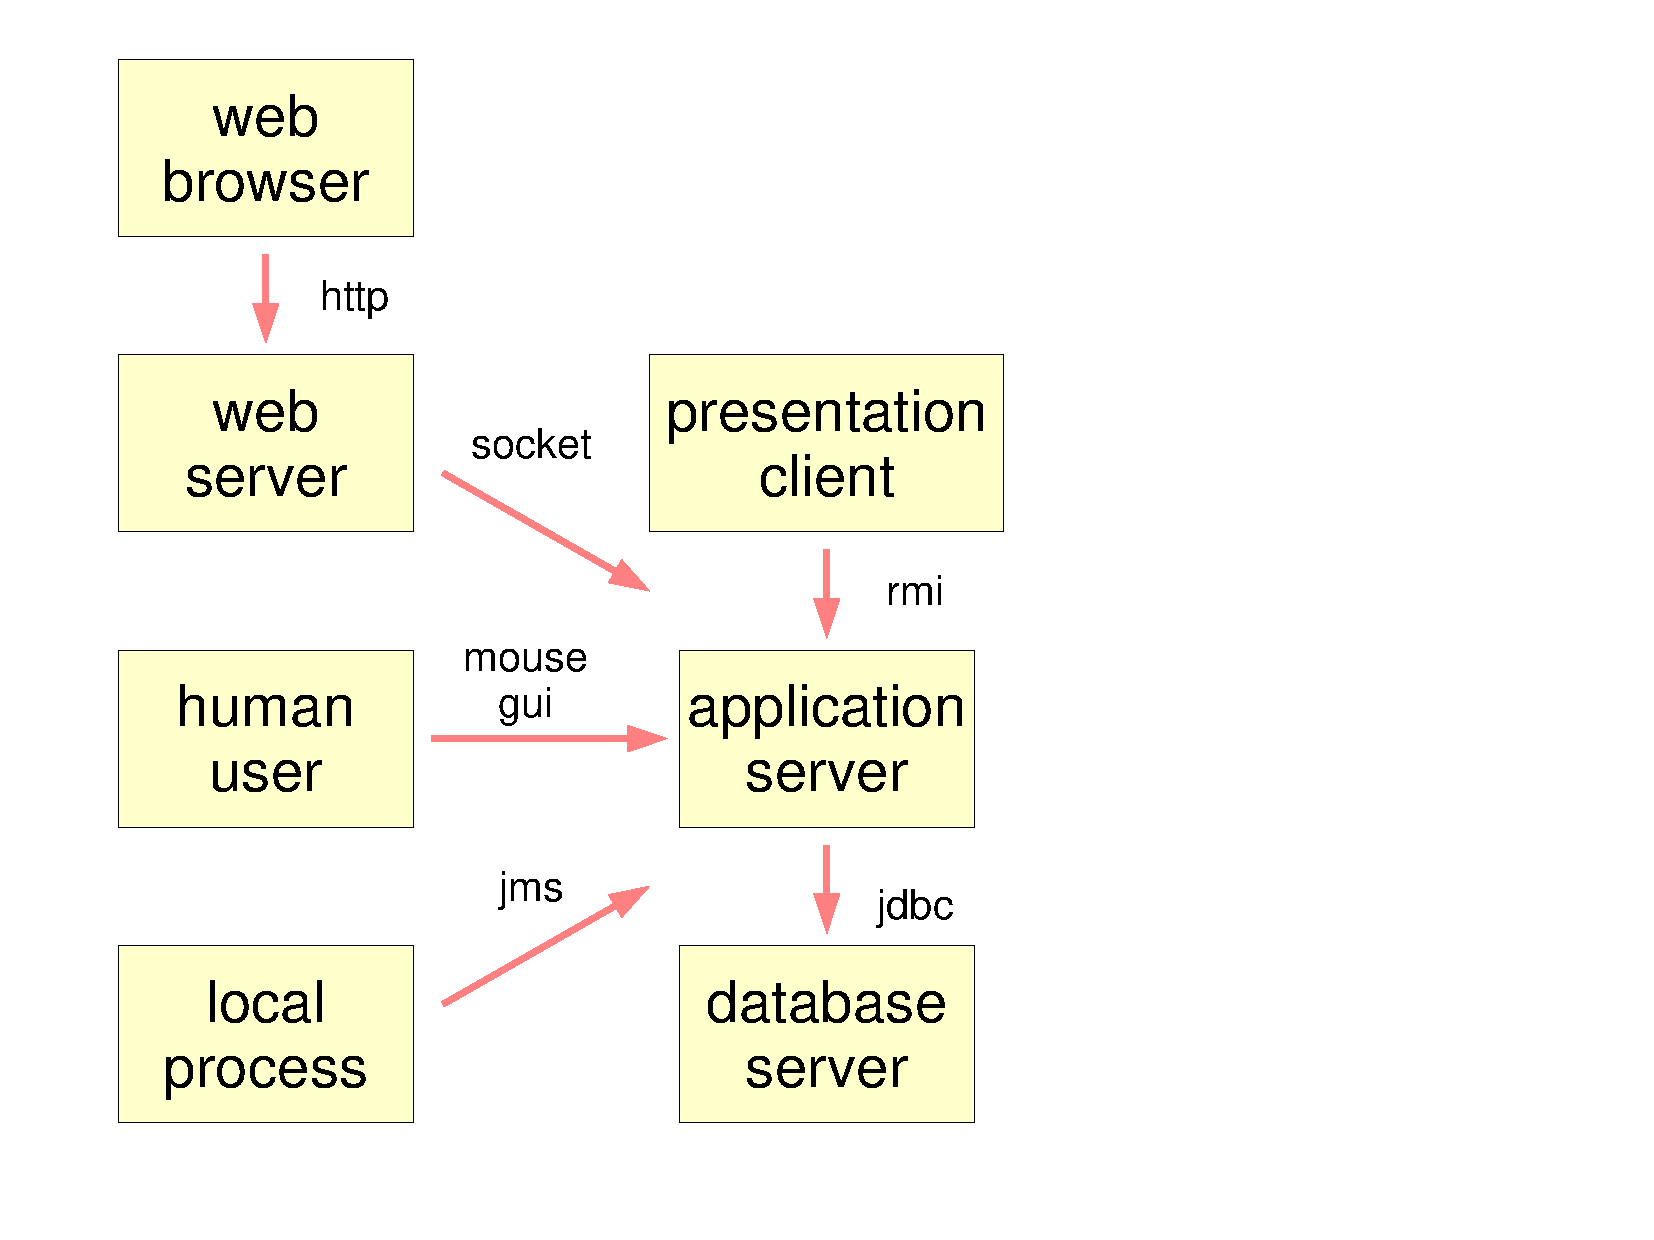
\includegraphics[scale=0.3,angle=-90]{graphic/user.pdf}
        \caption{Human User}
        \label{user_figure}
    \end{center}
\end{figure}

At the second view, one realises that due to the difference in construction,
human systems rely on other kinds of communication signals. While network cards
are usually enough for two computers to exchange data, additional input/ output
devices are needed to let human beings and computers talk to each other. To these
devices count: \emph{Keyboard}, \emph{Mouse}, \emph{Screen}, \emph{Printer} and
many more. They are made to suit the five human senses, that is to generate and
understand optical, acoustical, mechanical and similar signals.

The optical information displayed on a screen is often systematised into
character-based \emph{Textual User Interface} (TUI) and window-based
\emph{Graphical User Interface} (GUI).

The scientific subject dealing with those issues in more detail is called
\emph{Human-Computer Interaction} (HCI). One working definition given in
\cite{sigchi} states:

\begin{quote}
    Human-computer interaction is a discipline concerned with the design,
    evaluation and implementation of interactive computing systems for human
    use and with the study of major phenomena surrounding them.
\end{quote}

%
% $RCSfile: peer_node.tex,v $
%
% Copyright (C) 2002-2008. Christian Heller.
%
% Permission is granted to copy, distribute and/or modify this document
% under the terms of the GNU Free Documentation License, Version 1.1 or
% any later version published by the Free Software Foundation; with no
% Invariant Sections, with no Front-Cover Texts and with no Back-Cover
% Texts. A copy of the license is included in the section entitled
% "GNU Free Documentation License".
%
% http://www.cybop.net
% - Cybernetics Oriented Programming -
%
% http://www.resmedicinae.org
% - Information in Medicine -
%
% Version: $Revision: 1.1 $ $Date: 2008-08-19 20:41:08 $ $Author: christian $
% Authors: Christian Heller <christian.heller@tuxtax.de>
%

\section{Peer Node}
\label{peer_node_heading}
\index{Peer Node}
\index{Distributed System}
\index{Distributed Computing Environment}
\index{DCE}
\index{c/s}
\index{Peer-to-Peer}
\index{P2P}
\index{Client}
\index{Server}
\index{Freenet}
\index{Gnutella}
\index{BitTorrent}
\index{eDonkey}
\index{FastTrack}
\index{Napster}

Tanenbaum and Steen \cite{tanenbaum2002} define a \emph{Distributed System} as
\textit{a collection of independent computers that appear to its users as a
single coherent system}. With \emph{System} referring to a process rather than
only hardware, as defined in section \ref{process_heading}, it seems appropriate
to rephrase and use this for the definition of a general
\emph{Distributed Computing Environment} (DCE):

\begin{quote}
    A distributed computing environment consists of at least two systems that
    work together over a network but run on independent computer hardware (nodes).
\end{quote}

\begin{figure}[ht]
    \begin{center}
        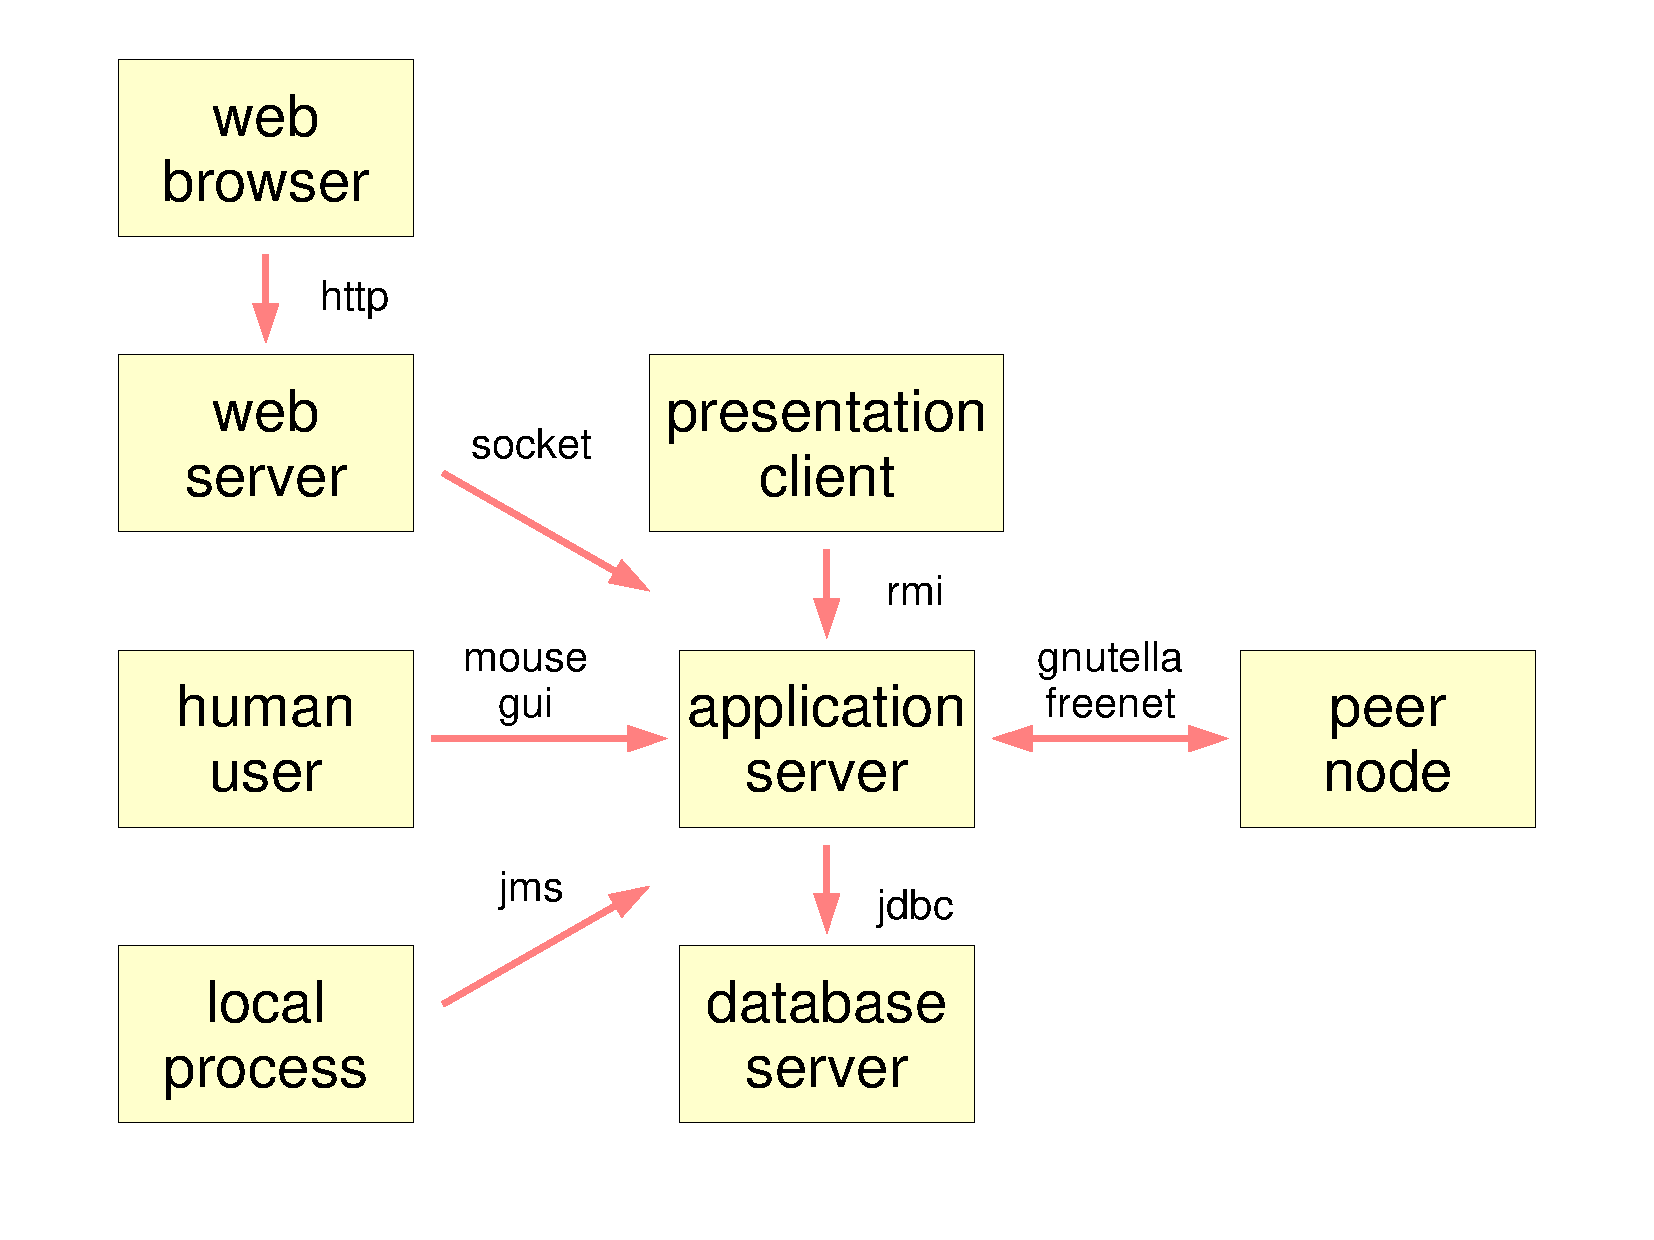
\includegraphics[scale=0.3,angle=-90]{graphic/peer.pdf}
        \caption{Peer-to-Peer Node Communication}
        \label{peer_figure}
    \end{center}
\end{figure}

Besides the previously mentioned client/ server (c/s) environments, so-called
\emph{Peer-to-Peer} (P2P) computer networks latterly became popular. In them,
nodes do not have just one role, but act as client and server at the same time
(figure \ref{peer_figure}), thus sharing their computing power and bandwidth.
Common P2P protocols are: \emph{Freenet}, \emph{Gnutella2}, \emph{BitTorrent},
\emph{eDonkey}, \emph{FastTrack} or \emph{Napster} \cite{wikipedia}. Many more
exist.

Just like nodes in a P2P network, human beings are capable of communicating
both ways, taking the role of a client or server. The organs that are needed to
do so are put into comparison with the corresponding devices of a computer
system, in chapter \ref{state_and_logic_heading}.

%
% $RCSfile: remote_server.tex,v $
%
% Copyright (C) 2002-2008. Christian Heller.
%
% Permission is granted to copy, distribute and/or modify this document
% under the terms of the GNU Free Documentation License, Version 1.1 or
% any later version published by the Free Software Foundation; with no
% Invariant Sections, with no Front-Cover Texts and with no Back-Cover
% Texts. A copy of the license is included in the section entitled
% "GNU Free Documentation License".
%
% http://www.cybop.net
% - Cybernetics Oriented Programming -
%
% http://www.resmedicinae.org
% - Information in Medicine -
%
% Version: $Revision: 1.1 $ $Date: 2008-08-19 20:41:08 $ $Author: christian $
% Authors: Christian Heller <christian.heller@tuxtax.de>
%

\section{Remote Server}
\label{remote_server_heading}
\index{Remote Server}
\index{Streams}
\index{Common Object Request Broker Architecture}
\index{CORBA}
\index{Simple Object Access Protocol}
\index{SOAP}
\index{Network Dynamic Data Exchange}
\index{NetDDE}
\index{Distributed Component Object Model}
\index{DCOM}
\index{COM+}
\index{KParts}
\index{Universal Network Objects}
\index{UNO}

Figure \ref{remote_figure} introduces a \emph{Remote Server} to the illustrated
example environment. It may access a database system -- similarly to the already
existing application server. In this example, however, it just works on simple
local files, using \emph{Streams}.

\begin{figure}[ht]
    \begin{center}
        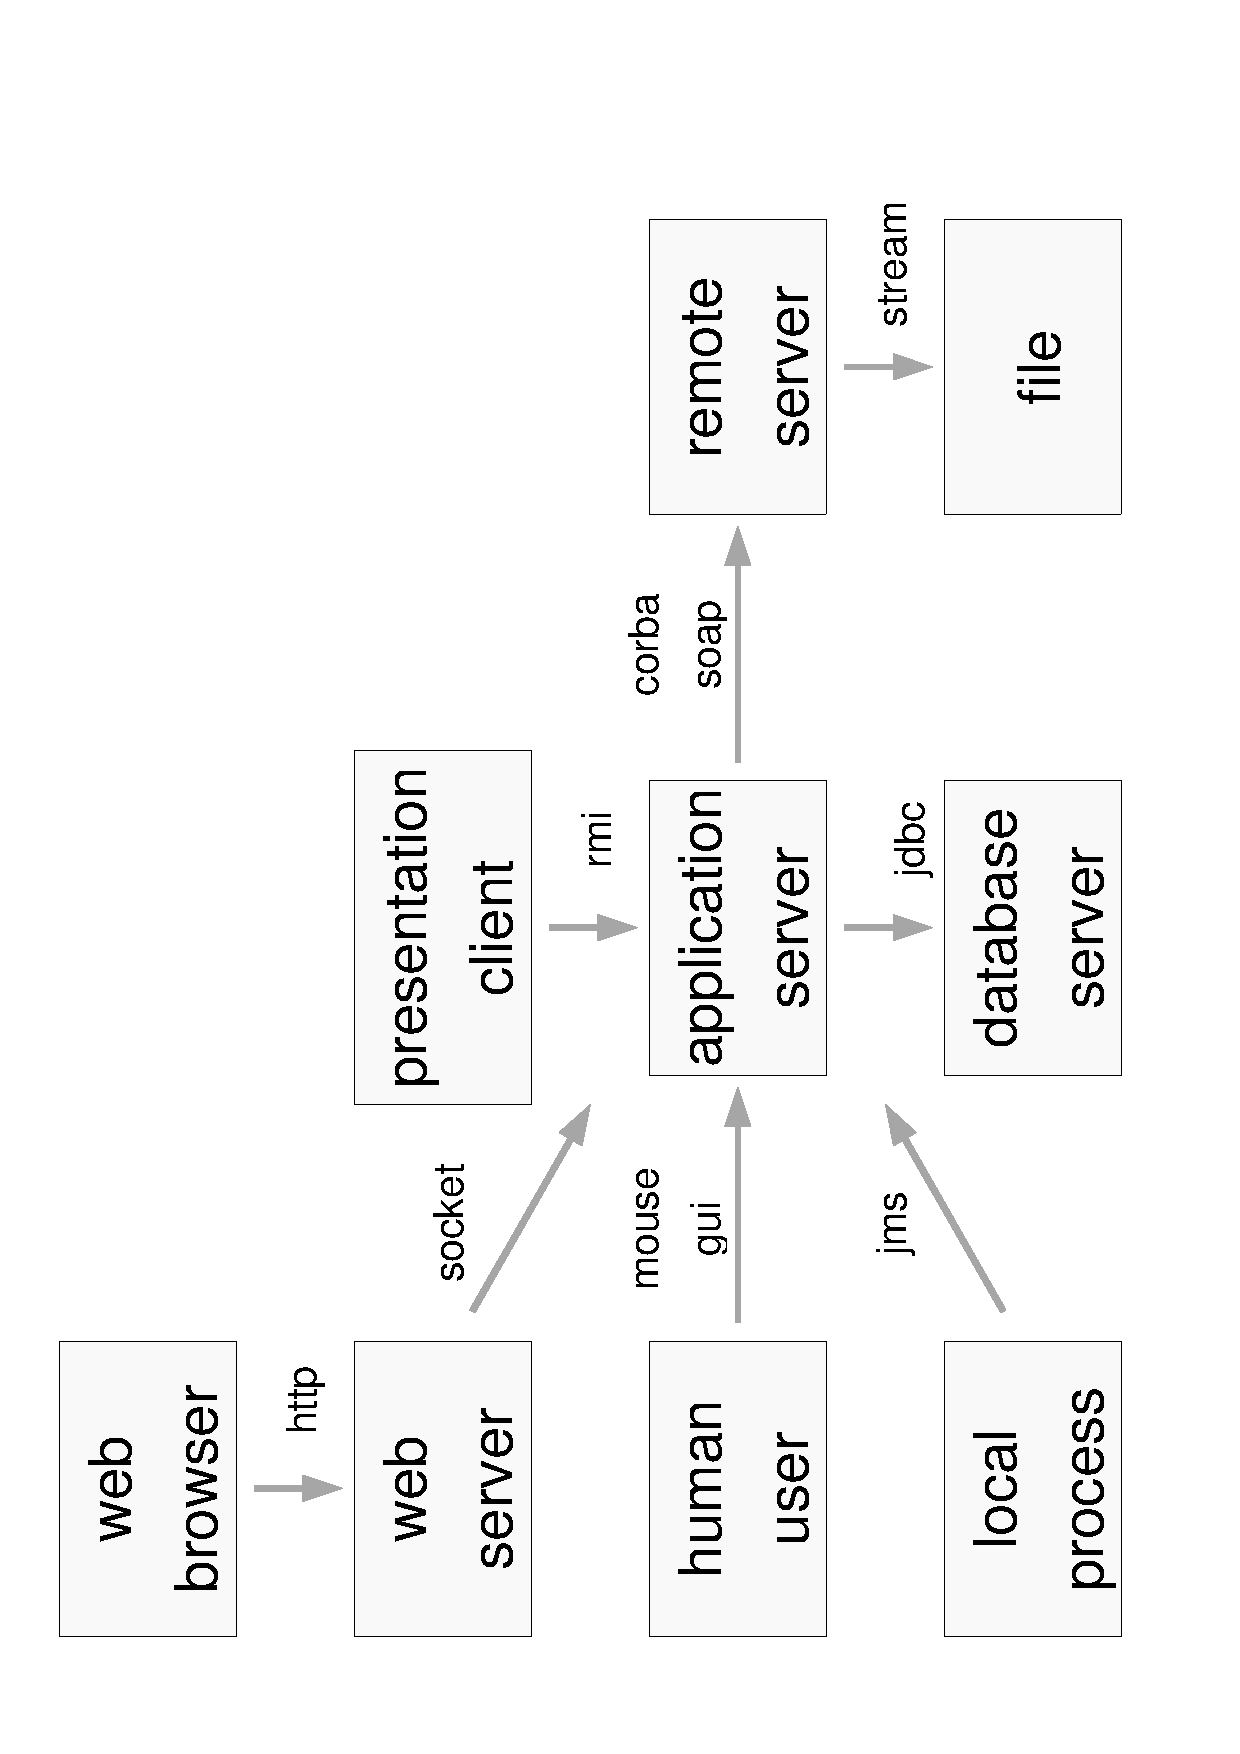
\includegraphics[scale=0.3,angle=-90]{graphic/remote.pdf}
        \caption{Remote Server}
        \label{remote_figure}
    \end{center}
\end{figure}

Like the previously introduced kinds of systems, remote systems need to rely on
a number of standards and mechanisms, in order to be able to communicate over
network. A comparison of some of these is given in \cite{olson, brownech, hrastnik}.
In the following is a list of common techniques that were not yet mentioned
before:

\begin{itemize}
    \item[-] \emph{Common Object Request Broker Architecture} (CORBA)
        \cite{corba, vinoski, gruhn}
    \item[-] \emph{Simple Object Access Protocol} (SOAP) \cite{soap}
    \item[-] \emph{Network Dynamic Data Exchange} (NetDDE) \cite{ddefaq}
    \item[-] \emph{Distributed Component Object Model} (DCOM/ COM+) \cite{gruhn}
    \item[-] \emph{KParts} \cite{kde}
    \item[-] \emph{Universal Network Objects} (UNO) \cite{openoffice}
\end{itemize}

%
% $RCSfile: legacy_host.tex,v $
%
% Copyright (C) 2002-2008. Christian Heller.
%
% Permission is granted to copy, distribute and/or modify this document
% under the terms of the GNU Free Documentation License, Version 1.1 or
% any later version published by the Free Software Foundation; with no
% Invariant Sections, with no Front-Cover Texts and with no Back-Cover
% Texts. A copy of the license is included in the section entitled
% "GNU Free Documentation License".
%
% http://www.cybop.net
% - Cybernetics Oriented Programming -
%
% http://www.resmedicinae.org
% - Information in Medicine -
%
% Version: $Revision: 1.1 $ $Date: 2008-08-19 20:41:07 $ $Author: christian $
% Authors: Christian Heller <christian.heller@tuxtax.de>
%

\section{Legacy Host}
\label{legacy_host_heading}
\index{Legacy Host}
\index{Legacy Systems}
\index{Host}
\index{Mainframe}
\index{Common Business Oriented Language}
\index{COBOL}
\index{Programming Language One}
\index{PL/I}
\index{Virtual Storage Access Method}
\index{VSAM}
\index{Third Party Maintenance}
\index{TPM}
\index{Customer Information Control System}
\index{CICS}

Finally, there is often a need to integrate \emph{Legacy Systems}, which are a
special variant of remote software systems running on computers with an older
architecture. Those computers are also named \emph{Host}, as in the example of
figure \ref{legacy_figure}, or \emph{Mainframe}. The applications running on
them are programmed in languages like the \emph{Common Business Oriented Language}
(COBOL) or \emph{Programming Language One} (PL/I) \cite{pli}, the latter
developed as an \emph{International Business Machines} (IBM) \cite{ibm} product
in the mid 1960's.

\begin{figure}[ht]
    \begin{center}
        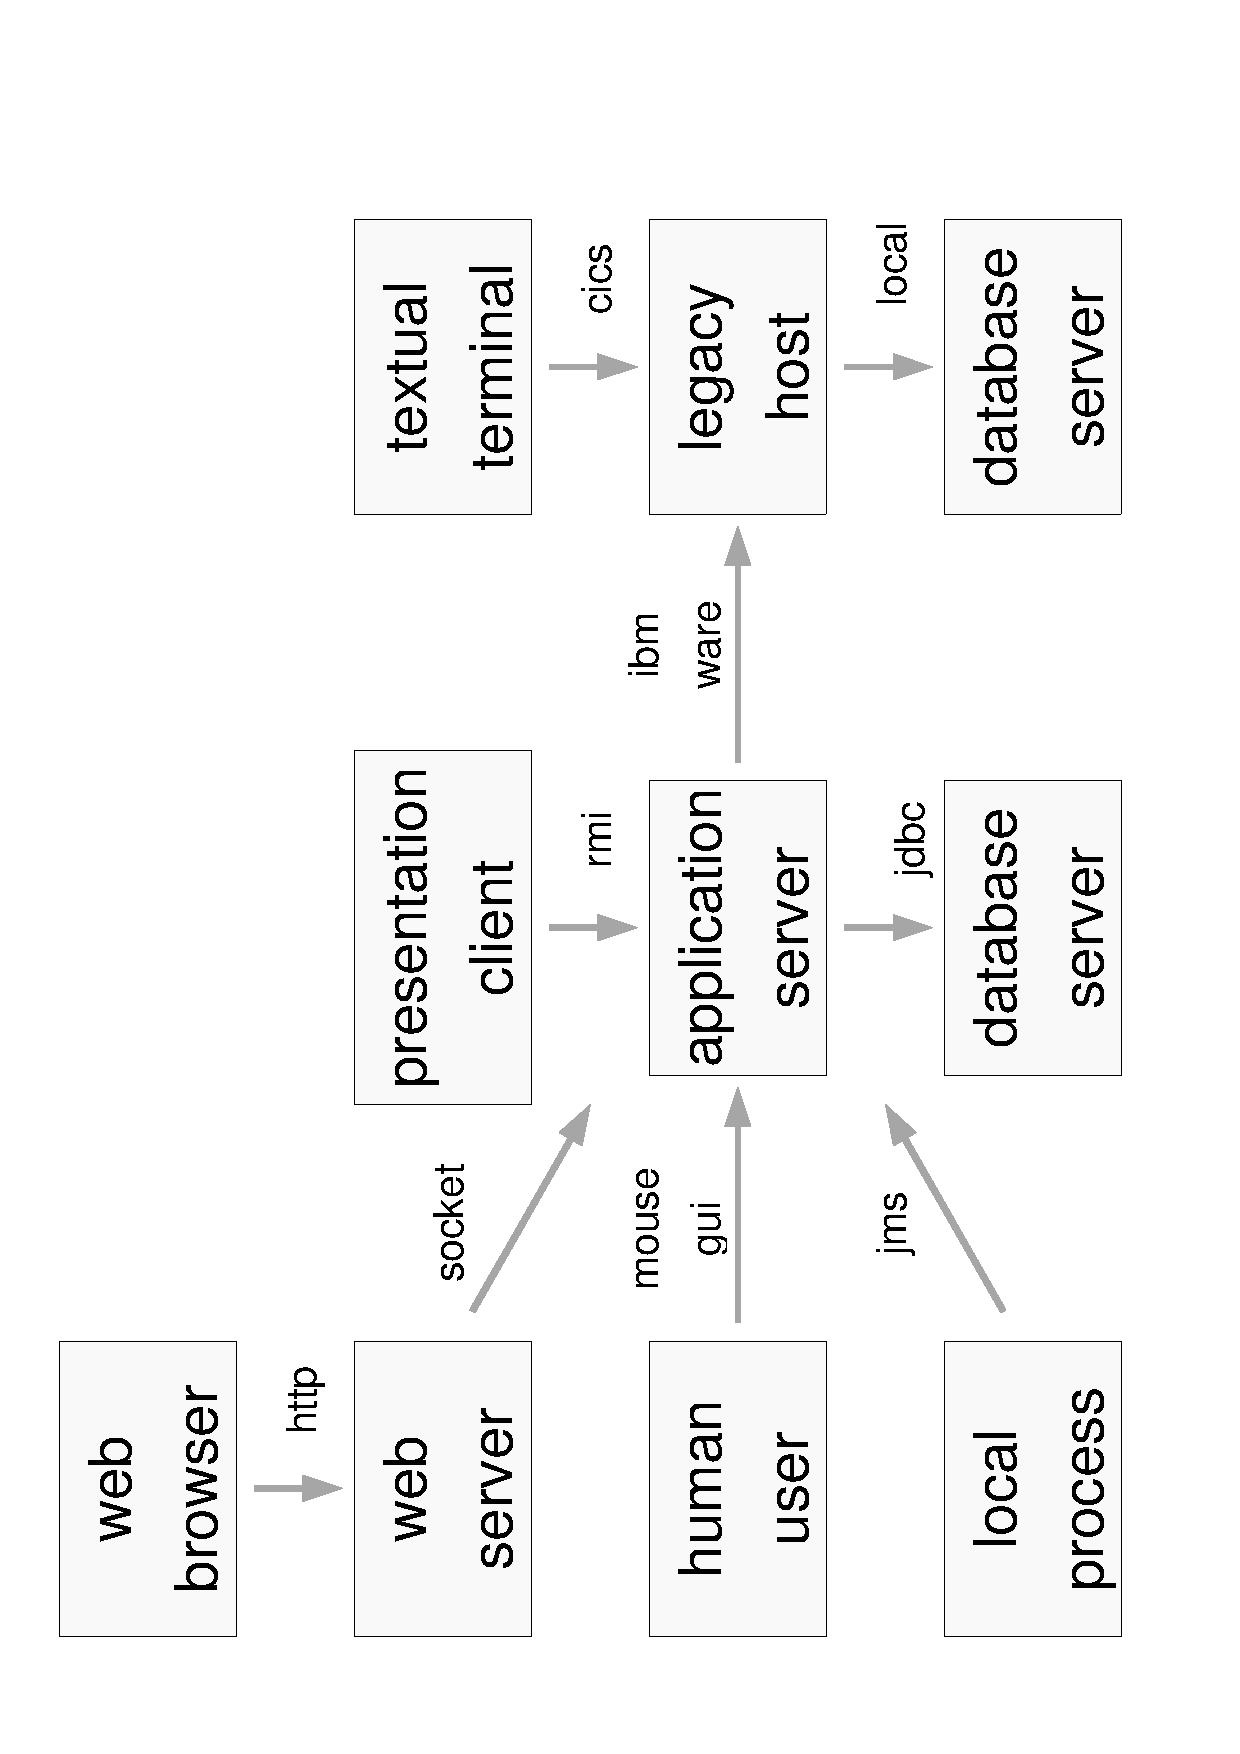
\includegraphics[scale=0.3,angle=-90]{graphic/legacy.pdf}
        \caption{Legacy Host}
        \label{legacy_figure}
    \end{center}
\end{figure}

Host computers manage nearly everything an ancient information technology
environment needs. They are responsible for persistence and processing of data.
Often, they contain hierarchical databases \cite{oolegacysystems} using flat
files like the \emph{Virtual Storage Access Method} (VSAM) format. True clients
do not exist here. Character-based terminals are the way to communicate with
the host which controls all interaction (including keyboard and screen), within
a \emph{Third Party Maintenance} (TPM) \emph{Customer Information Control System}
(CICS) runtime environment.

%
% $RCSfile: systems_interconnection.tex,v $
%
% Copyright (C) 2002-2008. Christian Heller.
%
% Permission is granted to copy, distribute and/or modify this document
% under the terms of the GNU Free Documentation License, Version 1.1 or
% any later version published by the Free Software Foundation; with no
% Invariant Sections, with no Front-Cover Texts and with no Back-Cover
% Texts. A copy of the license is included in the section entitled
% "GNU Free Documentation License".
%
% http://www.cybop.net
% - Cybernetics Oriented Programming -
%
% http://www.resmedicinae.org
% - Information in Medicine -
%
% Version: $Revision: 1.1 $ $Date: 2008-08-19 20:41:09 $ $Author: christian $
% Authors: Christian Heller <christian.heller@tuxtax.de>
%

\section{Systems Interconnection}
\label{systems_interconnection_heading}
\index{Systems Interconnection}
\index{Open Systems Interconnection}
\index{OSI}
\index{International Organization for Standardization}
\index{ISO OSI Reference Model}
\index{Simple Mail Transfer Protocol}
\index{SMTP}
\index{Telephone Network}
\index{Telnet}
\index{File Transfer Protocol}
\index{FTP}
\index{Hypertext Transfer Protocol}
\index{HTTP}
\index{Domain Name Service}
\index{DNS}
\index{X.226}
\index{Remote Procedure Call}
\index{RPC}
\index{Network Basic Input/ Output System}
\index{NetBIOS}
\index{Transfer Control Protocol}
\index{TCP}
\index{User Datagram Protocol}
\index{UDP}
\index{Transport Protocol Class 4}
\index{TP4}
\index{Sequence Package Exchange}
\index{SPX}
\index{Internet Protocol}
\index{IP}
\index{Internet Packet Exchange}
\index{IPX}
\index{Point-to-Point Protocol}
\index{PPP}
\index{Serial Line Internet Protocol}
\index{SLIP}
\index{Frame Relay}
\index{FR}
\index{X.25}
\index{Ethernet}
\index{Token Ring}
\index{Fiber Distributed Data Interface}
\index{FDDI}
\index{Ontology}
\index{Health Level Seven}
\index{HL7}
\index{TCP/IP}
\index{Universal Interactive Executive}
\index{UNIX}
\index{Operating System}
\index{OS}

Communication is essential to an IT environment as described before. To enable
and ease communication across different systems, special solutions have been
developed and accepted as \emph{de facto} or \emph{de jure} standards. One such
specification is the well-known \emph{Open Systems Interconnection} (OSI)
reference model, defined by the \emph{International Organization for Standardization}
(ISO). Numerous books \cite{tanenbaum2000} and documents on the web
\cite{payer} describe this model and its protocols.

\begin{figure}[ht]
    \begin{center}
        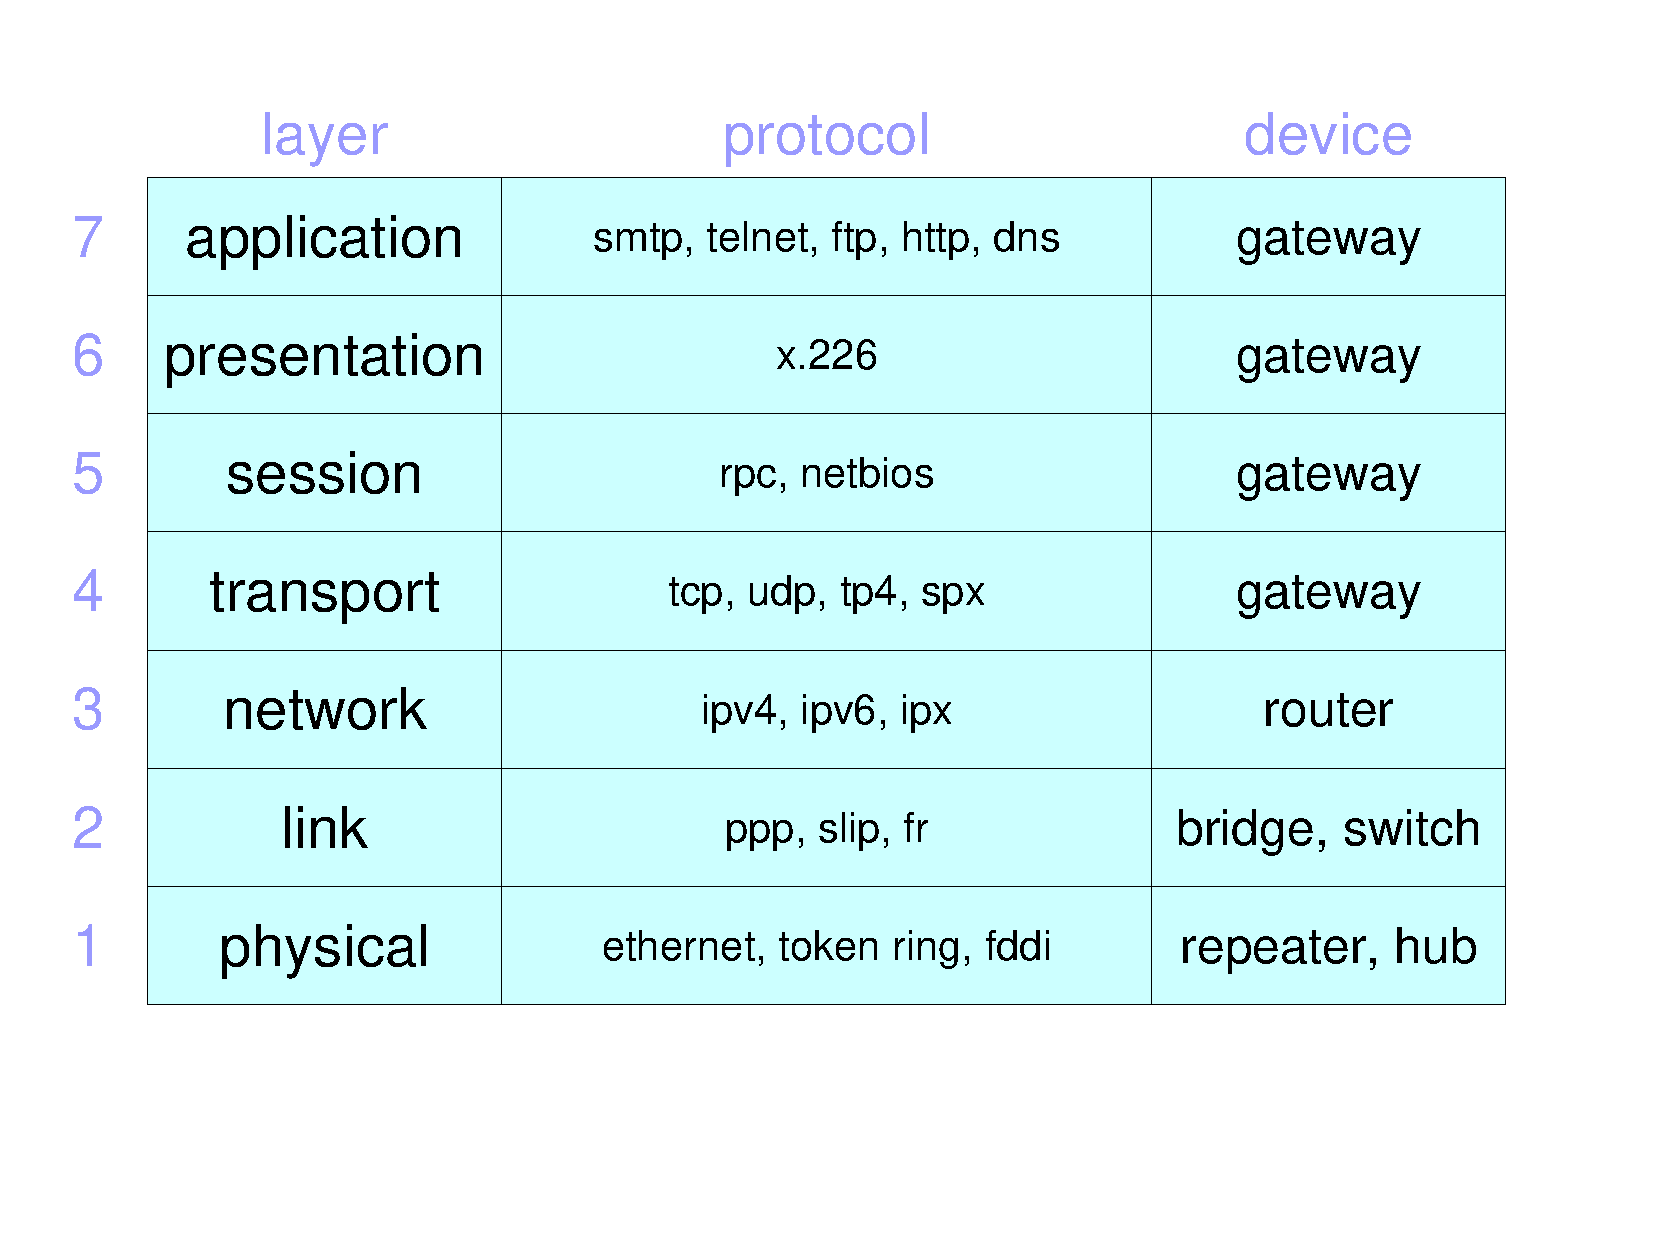
\includegraphics[scale=0.3,angle=-90]{graphic/osi.pdf}
        \caption{ISO OSI Reference Model}
        \label{osi_figure}
    \end{center}
\end{figure}

Figure \ref{osi_figure} organises the seven layers of the model in table form,
with one row representing one layer. The first column contains a layer's name,
the second examples of typical network protocols and the third devices in which
the protocols are used. \emph{Simple Mail Transfer Protocol} (SMTP),
\emph{Telephone Network} (Telnet), \emph{File Transfer Protocol} (FTP),
\emph{Hypertext Transfer Protocol} (HTTP) and \emph{Domain Name Service} (DNS)
are standard protocols used directly in software applications and -tools.
\emph{X.226} is a recommendation defining the OSI presentation protocol. The
\emph{Remote Procedure Call} (RPC) and \emph{Network Basic Input/ Output System}
(NetBIOS) may be sorted into the session layer. \emph{Transfer Control Protocol}
(TCP), \emph{User Datagram Protocol} (UDP), \emph{Transport Protocol Class 4}
(TP4) and \emph{Sequence Package Exchange} (SPX) do belong to the transport
layer. The \emph{Internet Protocol} (IP) is used in two versions: 4 and 6. Both
of them are situated on the network level of the OSI model, just like the
\emph{Internet Packet Exchange} (IPX) protocol. The link level contains the
\emph{Point-to-Point Protocol} (PPP), \emph{Serial Line Internet Protocol}
(SLIP) and \emph{Frame Relay} (FR), the latter being a replacement for veterans
like \emph{X.25}. To the physical level transmitting raw Bits finally, belong
\emph{Ethernet}, \emph{Token Ring} and \emph{Fiber Distributed Data Interface}
(FDDI).

Many of the mentioned protocols may be assigned to more than just one layer.
But it is \emph{not} the intention of this work to deal with such details. The
overall ISO OSI model, however, is mentioned because it is a good example of a
structure whose layers represent increasing levels of abstraction, what will
later in this work be called an \emph{Ontology} (chapters
\ref{logical_architecture_heading} and \ref{knowledge_schema_heading}). Also,
the \emph{Health Level Seven} (HL7) medical standard, which gets introduced in
chapter \ref{res_medicinae_heading}, received its name from referring to OSI's
seventh level -- the application level \cite{rogers}.

While the ISO OSI model defines seven abstract communication layers, the
popular \emph{TCP/IP} model uses solely four. Web communication as described in
section \ref{web_client_and_server_heading} is based on it. Today, TCP/IP has
become the standard in network management systems. A majority of them run the
\emph{Universal Interactive Executive} (UNIX) \emph{Operating System} (OS), of
which TCP/IP is an integral part. Margarete Payer \cite{payer} writes:
\textit{Although the OSI Model is affected with various deficiencies, it is
well suitable for didactic purposes.} Further, she mentions that since some
time, Andrew S. Tanenbaum uses a hybrid model for structuring his standard book
on computer networks \cite{tanenbaum2000}, which sticked to neither OSI nor
TCP/IP.

%
% $RCSfile: scalability.tex,v $
%
% Copyright (C) 2002-2008. Christian Heller.
%
% Permission is granted to copy, distribute and/or modify this document
% under the terms of the GNU Free Documentation License, Version 1.1 or
% any later version published by the Free Software Foundation; with no
% Invariant Sections, with no Front-Cover Texts and with no Back-Cover
% Texts. A copy of the license is included in the section entitled
% "GNU Free Documentation License".
%
% http://www.cybop.net
% - Cybernetics Oriented Programming -
%
% http://www.resmedicinae.org
% - Information in Medicine -
%
% Version: $Revision: 1.1 $ $Date: 2008-08-19 20:41:08 $ $Author: christian $
% Authors: Christian Heller <christian.heller@tuxtax.de>
%

\section{Scalability}
\label{scalability_heading}
\index{Scalability}
\index{Vertical Scaling}
\index{Horizontal Scaling}
\index{Symmetric Multiprocessing}
\index{SMP}
\index{Central Processing Units}
\index{CPU}
\index{Operating System}
\index{OS}
\index{Input/ Output}
\index{i/o}
\index{Reliability, Availability, Serviceability}
\index{RAS}
\index{Clustering}
\index{Vertical System}
\index{Horizontal System}
\index{Large Database}
\index{Web Server}
\index{Transactional Database}
\index{Firewall}
\index{Data Warehouse}
\index{Proxy Server}
\index{Data Mining}
\index{Directories}
\index{Application Server}
\index{High Performance Technical Computing}
\index{HPTC}
\index{Media Streaming}
\index{Extensible Markup Language Processing}
\index{XML}
\index{Java Server Pages Application}
\index{JSP}
\index{Secure Socket Layer}
\index{SSL}
\index{Virtual Private Network}
\index{VPN}
\index{Application Types}
\index{Interconnect}
\index{Loosely-coupled external Interconnect}
\index{Tightly-coupled internal Interconnect}

The previous sections demonstrated that there are many different ways to organise
a distributed information technology environment. The physical distribution of
systems is often a user requirement, either to connect different locations or to
reach better performance by sharing the work load. The degree to which a system
can be distributed to different hardware is often called its \emph{Scalability}.
Two models of scaling can be distinguished: \emph{vertical} and \emph{horizontal}
computing (figure \ref{scaling_figure}), whose key characteristics are only
described briefly here.

\begin{figure}[ht]
    \begin{center}
        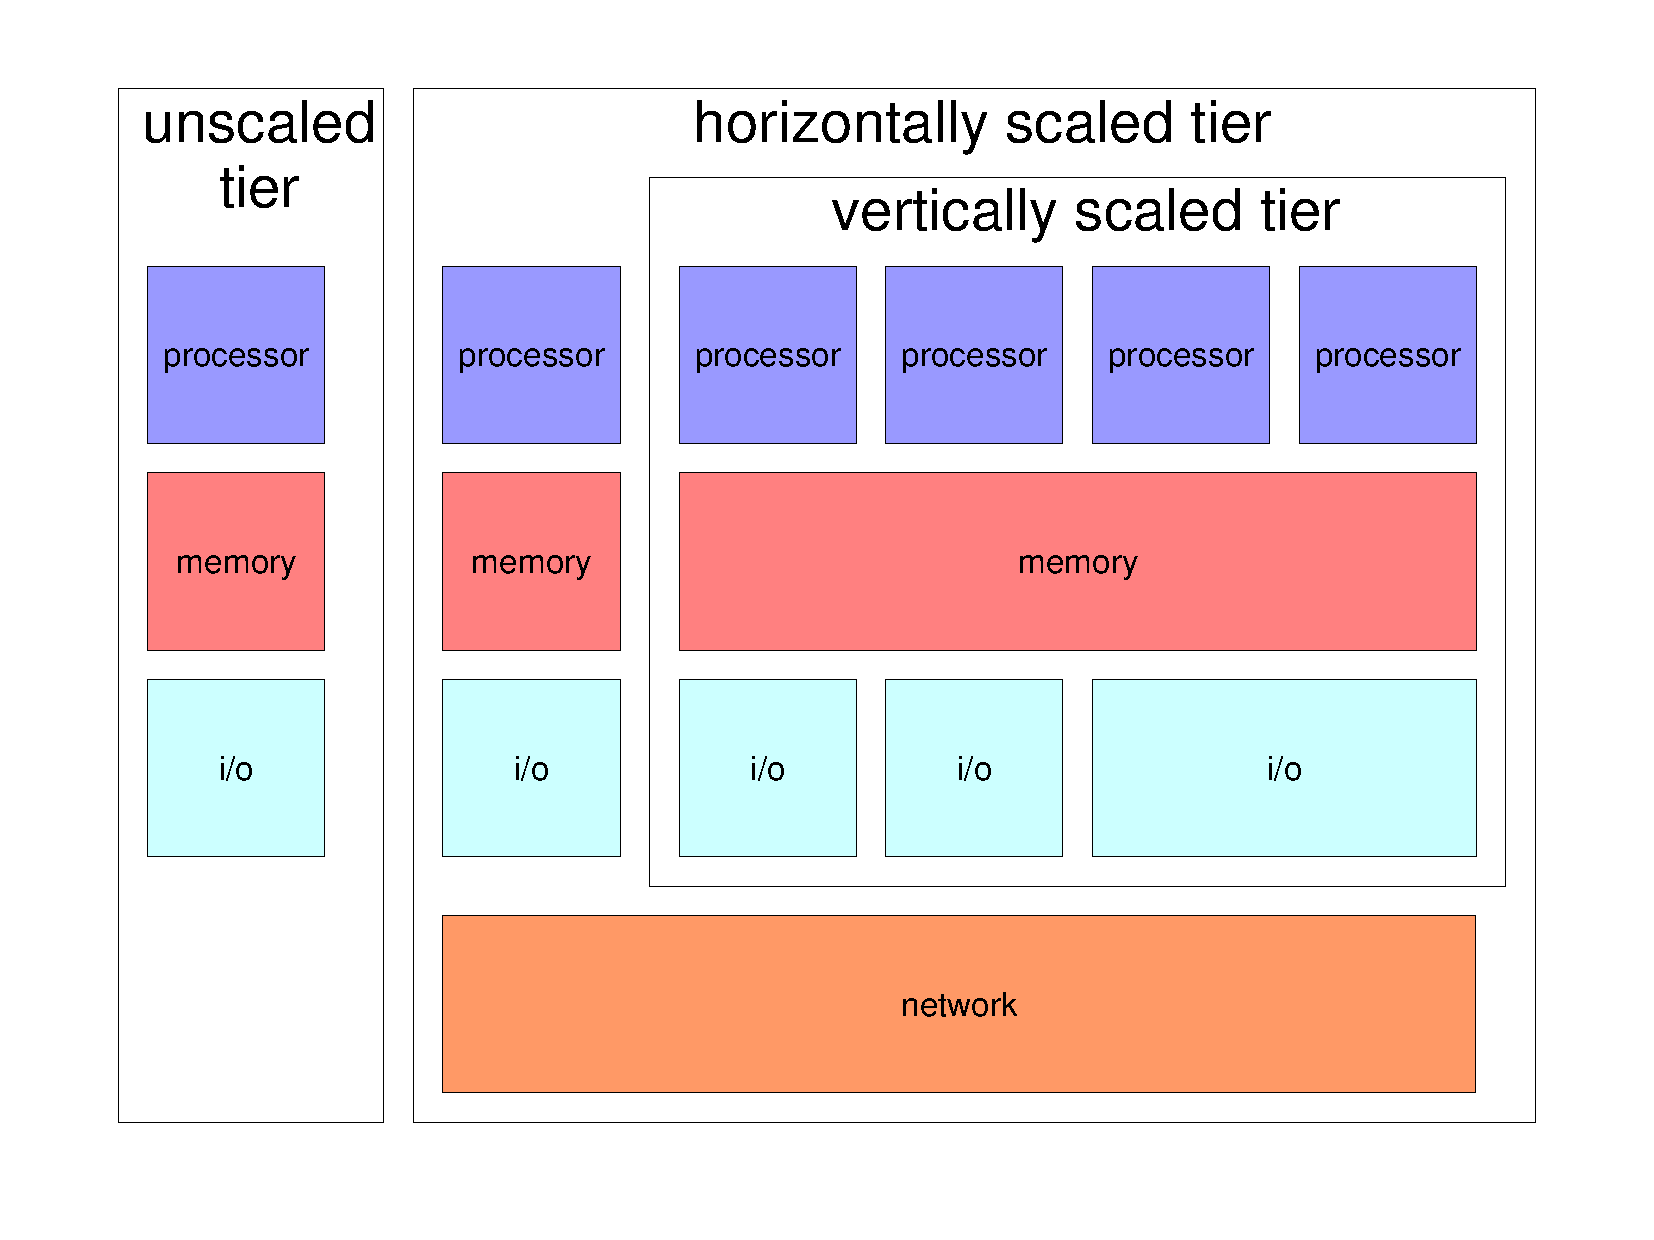
\includegraphics[scale=0.3,angle=-90]{graphic/scaling.pdf}
        \caption{Vertical and Horizontal Scaling}
        \label{scaling_figure}
    \end{center}
\end{figure}

Vertical servers are large \emph{Symmetric Multiprocessing} (SMP) systems with
more than four \emph{Central Processing Units} (CPU) that share one common memory.
One single \emph{Operating System} (OS) instance covers the processors, the memory
and input/ output (i/o) components. Vertical servers provide high availability by
building numerous \emph{Reliability, Availability, Serviceability} (RAS) features
into the individual server, to minimise un-/planned downtime.

The alternative horizontal scaling connects many systems over network, which is
often called \emph{Clustering}. A cluster contains computing nodes having one to
four processors and a memory each. The input/ output devices may belong to just
one node or be shared by many. Each node has an OS instance. \textit{Horizontal
servers do not build RAS features into the individual servers but get high RAS
by replication and deployment of many servers}, as Atwood \cite{atwood} writes.

\begin{table}[ht]
    \begin{center}
        \begin{footnotesize}
        \begin{tabular}{| p{50mm} | p{60mm} |}
            \hline
            \textbf{Vertical System} & \textbf{Horizontal System}\\
            \hline
            Large Database & Web Server\\
            \hline
            Transactional Database & Firewall\\
            \hline
            Data Warehouse & Proxy Server\\
            \hline
            Data Mining & Directories\\
            \hline
            Application Server & Application Server\\
            \hline
            High Performance Technical Computing (HPTC) application (non-partitionable) & High Performance Technical Computing (HPTC) application (partitionable)\\
            \hline
            & Media Streaming\\
            \hline
            & Extensible Markup Language (XML) Processing\\
            \hline
            & Java Server Pages (JSP) Application\\
            \hline
            & Secure Socket Layer (SSL)\\
            \hline
            & Virtual Private Network (VPN)\\
            \hline
        \end{tabular}
        \end{footnotesize}
        \caption{Vertical and Horizontal Application Types \cite{atwood}}
        \label{scalability_table}
    \end{center}
\end{table}

Table \ref{scalability_table} states some typical applications for vertical and
horizontal computing. The key difference, that after \cite{atwood} affected
both, their price and performance, is the \emph{Interconnect} used with each
architecture. Horizontal servers use a loosely-coupled \emph{external}
interconnect. Vertical servers use a tightly-coupled \emph{internal}
interconnect that makes data communications faster.

%
% $RCSfile$
%
% Copyright (c) 2005-2006. Christian Heller. All rights reserved.
%
% Permission is granted to copy, distribute and/or modify this document
% under the terms of the GNU Free Documentation License, Version 1.1 or
% any later version published by the Free Software Foundation; with no
% Invariant Sections, with no Front-Cover Texts and with no Back-Cover
% Texts. A copy of the license is included in the section entitled
% "GNU Free Documentation License".
%
% http://www.cybop.net
% - Cybernetics Oriented Programming -
%
% http://www.resmedicinae.org
% - Information in Medicine -
%
% Version: $Revision$ $Date$ $Author$
% Authors: Christian Heller <christian.heller@tuxtax.de>
%

\subsection{Misleading Tiers}
\label{misleading_tiers_heading}

When distinguishing human- and technical systems, the kinds of
\emph{Communication} are:

\begin{itemize}
    \item[-] Human $\leftrightarrow$ Human
    \item[-] Human $\leftrightarrow$ Computer
    \item[-] Computer $\leftrightarrow$ Computer
\end{itemize}

Each of these relies on different techniques, transport mechanisms, languages
(protocols) and so on. But the general principle after which communication
works, is always the same -- no matter whether technical \emph{Computer}
systems or their biological prototype, the \emph{Human Being}, are considered:
Information is \emph{received}, \emph{stored}, \emph{processed} and \emph{sent}.
Despite these common characteristics, today's \emph{Information Technology}
(IT) environments \cite{hellerkunze} treat communication between a computer
system and a human being differently than that \emph{among} computer systems.

\begin{figure}[ht]
    \begin{center}
        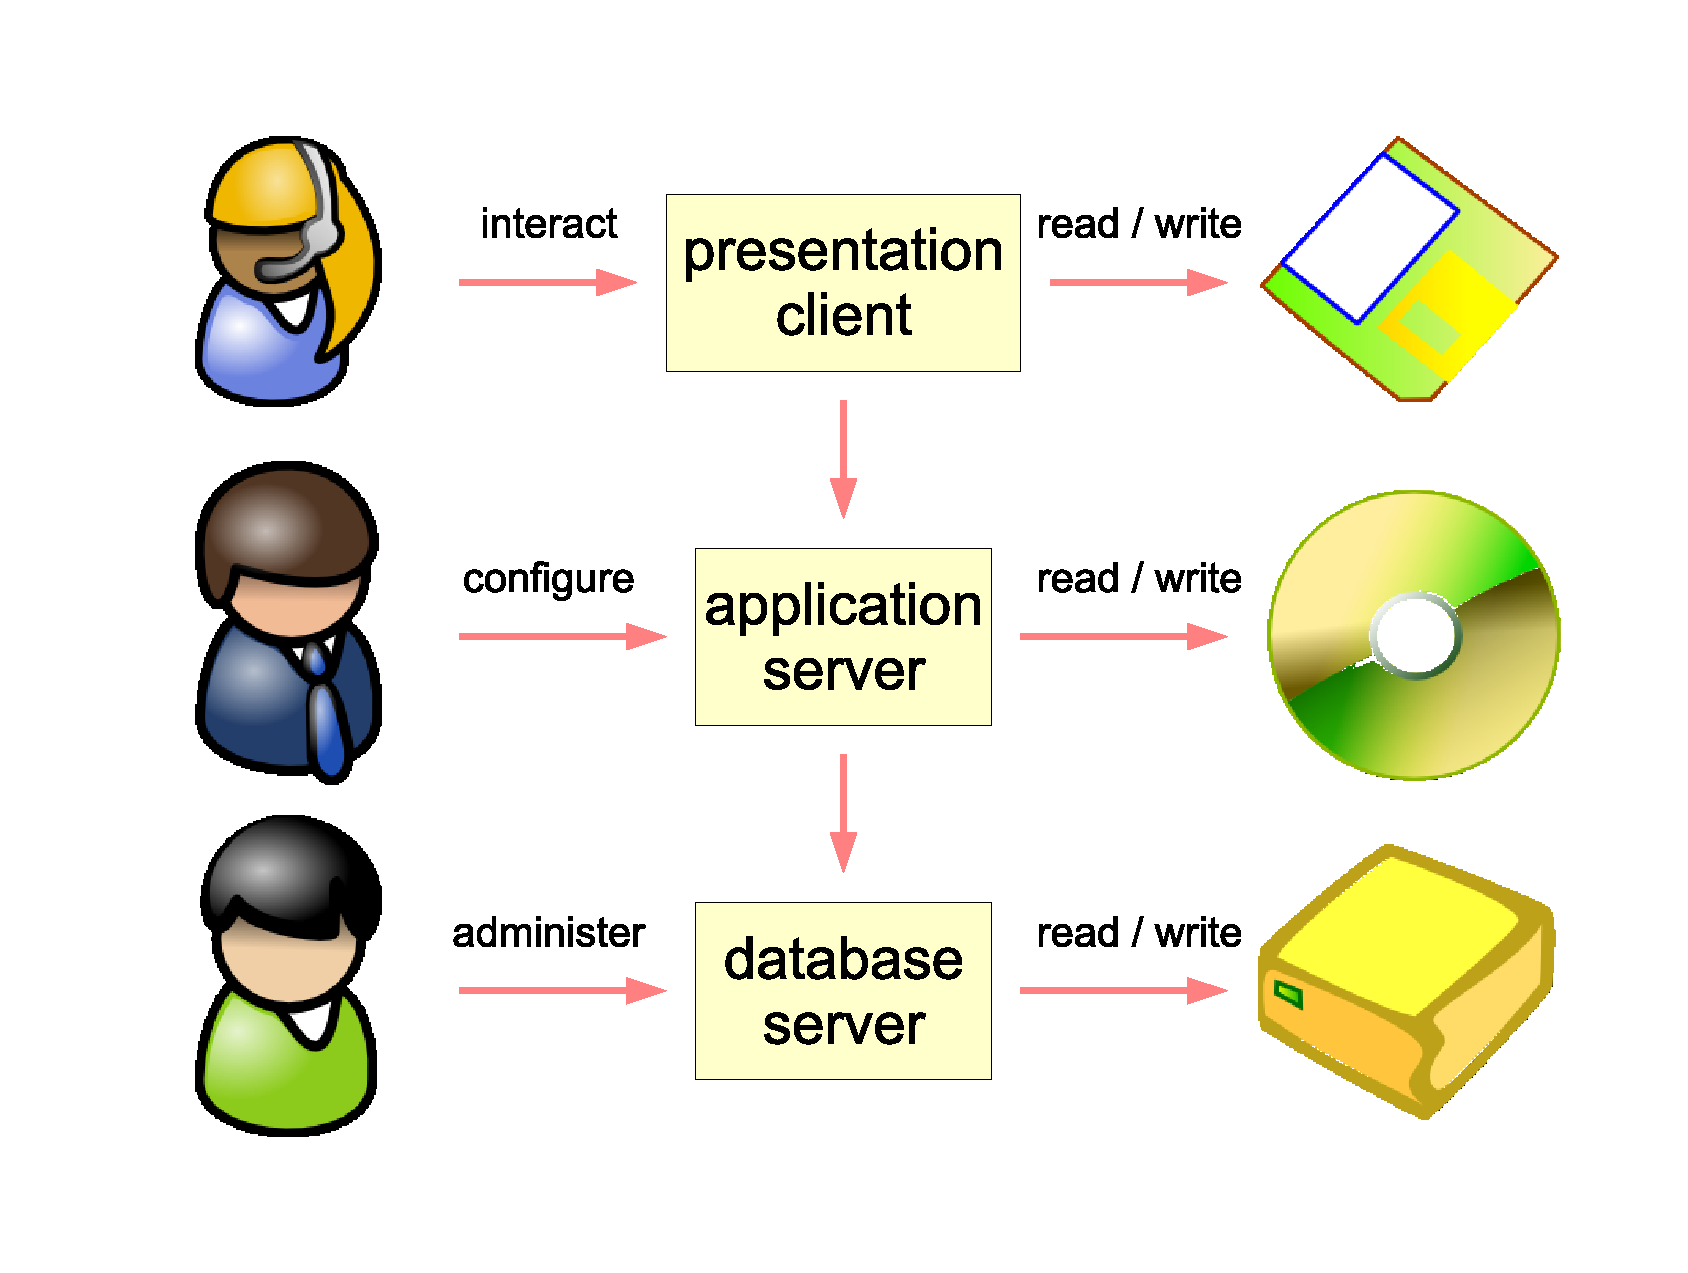
\includegraphics[scale=0.2]{vector/misleading.eps}
        \caption{Universal Communication}
        \label{misleading_figure}
    \end{center}
\end{figure}

Figure \ref{misleading_figure} shows a three-tier environment: tier 1 represents
the \emph{Presentation Layer}; tier 2 stands for the \emph{Application Layer};
tier 3 is the \emph{Database (DB) Layer}. Typical synonyms are, in this order:
\emph{Frontend}, \emph{Business Logic} and \emph{Backend}. The tiers (layers)
serve two needs: connect different locations and share work load (\emph{Scaling}).
However, the split into tiers of that kind raises two illusions:

\begin{enumerate}
    \item \emph{Users only interact with clients}
    \item \emph{Persistent data are stored in DB only}
\end{enumerate}

Many IT architectures, or at least their illustrations, neglect the fact that
in reality \emph{all} systems need a \emph{User Interface} (UI), for at least
being administered by humans, and \emph{almost} all systems, even
\emph{Database Management Systems} (DBMS) themselves, store some of their
persistent data outside a database, for example locally available configuration
information. This is not necessarily a problem for the IT environment as such,
but it is for the internal architecture of software systems. Special solutions
have to deal with frontend (UI framework), business logic (domain patterns) and
backend (data mapping), and often additional mechanisms for local and remote
communication. The serious differences in these design solutions are one root
of well-known problems like multi- directional inter-dependencies between system
parts, that make software difficult to develop and hard to maintain.

One aim of the work described in this article was to investigate possibilities
for a \emph{unification} of communication paradigms, that is high-level design
paradigms rather than low-level protocols, in order to architect software in a
way that allows the computer system it runs on to communicate \emph{universally}.

